\documentclass[12pt, openany]{book}

% This is all the packages and settings and so on.
% It is using custom fonts that needs to be installed on the computer. If they are not present, they have to be added manually.
\usepackage[
	citestyle=ieee, 
    bibstyle=ieee,
    style=numeric-comp,
    sorting=nty,
    maxbibnames=99, % Make sure we are printing all authors in the appendix
    ]{biblatex}
    
% Makes the last name first in the bibliography.
% \DeclareNameAlias{author}{last-first}
\DeclareNameAlias{author}{family-given}
    
% Specify the margins. This is 6.25inches in text with which 
% can be used to size figures to the correct size.
\usepackage[a4paper, margin=2.5625cm]{geometry}

\usepackage{eso-pic}					% Packages for layout and graphics 
\usepackage{graphicx}
\usepackage{tikz}
\usetikzlibrary{fadings}
\usepackage{setspace}
% \usepackage{tocloft}		 			% Fixing a bug with page style changes for toc
% \tocloftpagestyle{plain}
\usepackage{etoc} 						% Separate tocs for appendix and the rest    
\usepackage{chngcntr}					% Count figures within chapters
\usepackage{booktabs}					% Table formatting
\usepackage{fancyhdr}					% Setting the style for header and footer.
\usepackage{tabularx}
\usepackage{multirow}                   % For better tables 
\usepackage[hidelinks]{hyperref}		% Clickable links
\usepackage{nameref}					% References with names
\usepackage[parfill]{parskip}			% New line instead of indent for sections
\usepackage{tcolorbox}					% Create boxes around content
\tcbset{colback=white,arc=0mm}

\usepackage{amsmath}
\usepackage{mathdots}
\usepackage{yhmath}
\usepackage{siunitx}
\usepackage{array}
\usepackage{gensymb}
\usepackage{amssymb}
\usepackage{mathtools}              % Add text to math arrows.

\usepackage{cancel}
\usepackage{color}
\usepackage{multirow}
\usepackage{textcomp}               % Fixing warning for gensyb \perthousand
\usepackage{svg}                    % including svg files
\usepackage{caption}                % For subfigures
\usepackage{subcaption}
\usepackage{fontspec}
\usepackage{sectsty}
\usepackage{tocloft}

\usepackage[printonlyused]{acronym}


\counterwithin{figure}{section} 
\counterwithin{table}{section}

% Specifying fonts
\setmainfont{Georgia} 
\setsansfont{Arial}
\newfontfamily\footerfont{Georgia}

\chapterfont{\sffamily\fontsize{17}{17}}
\sectionfont{\sffamily\fontsize{14}{15}}
\subsectionfont{\sffamily\fontsize{13}{15}}
\subsubsectionfont{\sffamily\fontsize{12}{15}}

% Remove the title and make sure that the text is adjusted
% \usepackage{abstract}
% \setlength{\absleftindent}{0mm}
% \renewcommand{\abstractname}{\vspace{-\baselineskip}}
% \renewcommand{\abstractnamefont}{\sffamily\fontsize{14}{15}}
% \renewcommand{\abstracttextfont}{\normalfont\fontsize{12}{13}}

% Renaming and setting style of table of contents
\renewcommand*\contentsname{Contents}
\renewcommand*\cfttoctitlefont{\fontsize{16}{0}\bf\sffamily}
\renewcommand\cftchapfont{\fontsize{14}{0}\bf\sffamily}
\renewcommand\cftchappagefont{\fontsize{13}{0}\bf\sffamily}
\renewcommand\cftsecfont{\fontsize{12}{0}\sffamily}
\renewcommand\cftsecpagefont{\fontsize{12}{0}\sffamily}
\renewcommand\cftsubsecfont{\fontsize{12}{0}\sffamily}
\renewcommand\cftsubsecpagefont{\fontsize{12}{0}\sffamily}

% Styling the header and footer
\fancyhf{}
\fancyhead{}
\fancyfoot{}
\fancyhead[L]{\fontsize{11}{10}\selectfont\leftmark}
\fancyfoot[R]{\footerfont\thepage}
\setlength{\headheight}{15.5pt}


\fancypagestyle{plain}{
    \fancyhf{}
    \fancyhead{}
    \fancyfoot{}
    \renewcommand{\headrulewidth}{0pt}
    \fancyfoot[R]{\footerfont\thepage}
}

\pagestyle{fancy}

% Making the command for placing text in random locations
\newcommand\PlaceText[3]{%
\begin{tikzpicture}[remember picture,overlay]
\node[outer sep=0pt,inner sep=0pt,anchor=south west] 
  at ([xshift=#1,yshift=-#2]current page.north west) {#3};
\end{tikzpicture}%
}

% Disable hyphenation
\pretolerance=10000
\tolerance=2000 
\emergencystretch=50pt


% Defining files for bibliography
%\addbibresource{ref.bib}
\addbibresource{references.bib}

% Add a second bibliography file for the second author to allow
% both to update it through the Mendeley integration.
% \addbibresource{ref-author-2.bib}

% Defining document information
\title{Unsupervised 3D Human Pose Estimation}
\newcommand{\subtitle}{KTH Thesis Report \\ Draft for final thesis meeting}
\author{Sri Datta Budaraju}

\begin{document}
\setstretch{1.4}

% The front page of the document
\pagenumbering{roman}
\makeatletter
\begin{titlepage}

\vspace*{-4.6\baselineskip}
\hspace*{-0.15\textwidth}
\includegraphics[width=0.2\paperwidth]{setup/img/kth-logo.jpg}
\par\vspace*{2.5\baselineskip}

\PlaceText{65mm}{12mm}{\fontsize{12}{0}\sffamily DEGREE PROJECT IN COMPUTER SCIENCE AND ENGINEERING,}
\PlaceText{65mm}{17mm}{\fontsize{12}{0}\sffamily SECOND CYCLE, 30 CREDITS}
\PlaceText{65mm}{22mm}{\fontsize{12}{0}\sffamily\itshape STOCKHOLM, SWEDEN \the\year}

~\\

\makebox[0pt][l]{%
\begin{minipage}[b]{0.25\textwidth}
~\\
\end{minipage}
\begin{minipage}{0.65\textwidth}
\begin{flushleft}
{\fontsize{28}{24}\bf\sffamily\@title\\}
\vspace{1cm}
{\fontsize{19}{17}\bf\sffamily \subtitle\\}
\vspace{1cm} 
{\fontsize{16}{18}\sffamily \@author}\\
\end{flushleft}
\end{minipage}
}


% \hspace*{-3cm}\begin{minipage}[b]{63.5mm}
% ~\\
% \end{minipage}
% \begin{minipage}{0.65\textwidth}
% \begin{flushleft}
% {\fontsize{28}{24}\bf\sffamily\@title\\}
% \vspace{0.5cm}
% {\fontsize{19}{17}\bf\sffamily \subtitle\\}
% \vspace{0.5cm} 
% {\fontsize{16}{0}\sffamily \@author}\\
% \end{flushleft}
% \end{minipage}


\AddToShipoutPictureBG*{%]
    \AtPageLowerLeft{%
        
\includegraphics[width=1.0\paperwidth]{setup/img/kth-footer.png}
    }%
}

\PlaceText{70mm}{280mm}{\color{white}\fontsize{12}{0}\sffamily KTH ROYAL INSTITUTE OF TECHNOLOGY }
\PlaceText{70mm}{285mm}{\color{white}\fontsize{8}{0}\sffamily SCHOOL OF ELECTRICAL ENGINEERING AND COMPUTER SCIENCE }
\end{titlepage}
\makeatother

\newpage
\newpage
\thispagestyle{plain}
~\\
\vfill
{ \setstretch{1.1}
    \subsection*{Authors}
    Sri Datta Budaraju <budaraju@kth.se>\\
    School of Electrical Engineering and Computer Science\\
    KTH Royal Institute of Technology
    
    \subsection*{Place for Project}
    Stockholm, Sweden\\
    Stuttgart, Germany

    \subsection*{Examiner}
    Danica Kragic Jensfelt\\
    Stockholm, Sweden\\
    KTH Royal Institute of Technology
    
    \subsection*{Supervisor }
    Hedvig Kjellström\\
    Stockholm, Sweden\\
    KTH Royal Institute of Technology
    
    \subsection*{Supervisor - Host}
    Arij Bouazizi\\
    Stuttgart, Germany\\
    Mercedes-Benz AG,  Research and Development
    ~
}

% TODO -- uncomment
\newpage
\thispagestyle{plain}
%%%%%%%%%%%%%%%%%%%%%%%%%%%%%%%%%%%%
%%  The English abstract          %%
%%%%%%%%%%%%%%%%%%%%%%%%%%%%%%%%%%%%
\chapter*{Abstract}
%%%%%%%%%%%%%%%%%%%%%%%%%%%%%%%%%%%%

The thesis proposes an unsupervised representation learning method to predict 3D human pose from a 2D skeleton via a VAE-GAN hybrid network. The method learns to lift poses from 2D to 3D using self-supervision and adversarial learning techniques. The method does not use images, heatmaps, 3D pose annotations, paired/unpaired 2D-to-3D skeletons, 3D priors, synthetic 2D skeletons, multi-view or temporal information in any shape or form. The 2D skeleton input is taken by a VAE that encodes it in a latent space and then decodes that latent representation to a 3D pose. The 3D pose is then reprojected to 2D for a constrained, self-supervised optimization using the input 2D pose. Parallelly, the 3D pose is also randomly rotated and reprojected to 2D to generate a 'novel' 2D view for unconstrained adversarial optimization using a discriminator network. The combination of the optimizations of the original and the novel 2D views of the predicted 3D pose results in a 'realistic' 3D pose generation. The thesis shows that the encoding and decoding process of the VAE addresses the major challenge of erroneous and incomplete skeletons from 2D detection networks as inputs and that the variance of the VAE can be altered to get various plausible 3D poses for a given 2D input. Additionally, the latent representation could be used for cross-modal training and many downstream applications. The results on Human3.6M datasets outperform previous unsupervised approaches with less model complexity while addressing more hurdles in scaling the task to the real world.


\subsection*{Keywords}
Computer Vision, Projective Geometry, Deep Learning, Unsupervised Learning, 3D Human Pose Estimation, GAN, AutoEncoder, Hybrid Generative Model, Self-Supervision
% uncomment

% TODO -- uncomment
\newpage
\thispagestyle{plain}
%%%%%%%%%%%%%%%%%%%%%%%%%%%%%%%%%%%%
%%   The Swedish abstract         %%
%%%%%%%%%%%%%%%%%%%%%%%%%%%%%%%%%%%%
\chapter*{Abstract} 
%%%%%%%%%%%%%%%%%%%%%%%%%%%%%%%%%%%%
**YET TO BE TRANSLATED**


Svenskt abstract 
Svensk version av abstract – samma titel på svenska som på engelska.

Skriv samma abstract på svenska. Introducera ämnet för projektet och beskriv problemen som löses i materialet. Presentera 

\subsection*{Nyckelord}
Kandidat examensarbete, ...
% uncomment

\newpage
\thispagestyle{plain}
\chapter*{Acknowledgements}

I would like to express my sincere gratitude to my supervisor at KTH, Hedvig Kjellström, and my industrial supervisor, Arij Bouazizi for their patient guidance, encouragement, and constructive critique of this research work. I am thankful to my examiner, Danica Kragic Jensfelt for her feedback and evaluation of this thesis. I would like to thank Mercedes Benz for hosting my thesis and providing me with the required infrastructure. I would like to express my appreciation to Ulrich Kressel and Julian Wiederer for welcoming me to their research group. I would like to acknowledge the helpful feedback, support, and company from my thesis group at KTH and would like to thank Ruibo Tu, Jade Cock, and Oscar Örnberg for their immense help. I am thankful to my friends Nik Vaessen and Vivek Chalumuri for their helpful discussions, comments, and advice throughout the whole process. Finally, I am grateful to my family for their lifelong support. This thesis was carried out during a period of unprecedented uncertainty and was only possible as a result of the incredible patience and empathy shown by everyone involved in the process.   

\newpage

\chapter*{Acronyms}

\begin{acronym}[TBD]
    \acro{ann}[ANN]{Artificial Neural Network}
    \acro{ar/vr}[AR/VR]{Augmented Reality/Virtual Reality}
    \acro{hpe}[HPE]{Human Pose Estimation}
    \acro{kld}[KLD]{Kullback–Leibler Divergence}
    \acro{l1}[L1]{Least Absolute Deviations}
    \acro{mmvae}[MMVAE]{Mixture-of-Experts Multimodal Variational Auto-Enocder}
    \acro{mpjpe}[MPJPE]{Mean Per Joint Position Estimate}
    \acro{pjpe}[PJPE]{Per Joint Position Estimate}
    \acro{mse}[MSE]{Mean Squared Error}
    \acro{mvae}[MVAE]{Multimodal Variational Auto-Enocder}
    \acro{mocap}[MoCap]{Motion Capture}
    \acro{nrsfm}[NRSfM]{Non-Rigid Structure from Motion}
    \acro{pov}[POV]{Point of View}
    \acro{rgb}[RGB]{Red Green Blue}
    \acro{sota}[SOTA]{State-of-The-Art}
    \acro{umap}[UMAP]{Uniform Manifold Approximation and Projection}
    \acro{vae}[VAE]{Variational Auto-Encoder}
    \acro{gan}[GAN]{Generative Adversarial Network}
    \acro{wgan}[WGAN]{Wasserstein Generative Adversarial Network}
    \acro{wgangp}[WGAN-GP]{\ac{wgan} with Gradient Penalty}
    \acro{jsd}[JS-divergence]{Jensen–Shannon Divergence}
    \acro{emd}[EM distance]{Earth Mover's Distance}
    \acro{bvae}[$\boldsymbol{\beta}$-VAE]{Beta Variational Auto-Encoder}
    \acro{fc}[FC]{Fully Connected}
    \acro{relu}[ReLU]{Rectified Linear Unit}
    
\end{acronym}



\newpage

\etocdepthtag.toc{mtchapter}
\etocsettagdepth{mtchapter}{subsection}
\etocsettagdepth{mtappendix}{none}
\thispagestyle{plain}
\tableofcontents

\newpage




\pagenumbering{arabic}

\chapter{Introduction}
\label{chap:introduction}
With rapid advancements in deep learning facilitated by the developments in computational hardware, there has been tremendous growth in computer vision research and its applications \cite{AIandCompute}. One of the major tasks of computer vision that is required for real-world applications is to perceive and understand dynamic objects and more importantly humans.  

Human Pose Estimation, also referred to as HPE is a fundamental problem in computer vision that also forms a basis for human action and gesture recognition as well as human motion prediction. \ac{HPE} is defined as the localization of human joints (also known as keypoints, including head, eyes, ears, nose etc) mainly in images and videos in either a 2D or 3D coordinate space. The widely available and used data like images and videos are 2-dimensional data and lack spatial information which is crucial for most of the applications like autonomous driving, \ac{AR/VR}, social robots etc. Hence this thesis focus is on 3D Human Pose Estimation.

% Link things together with references. This is a reference to a section: \ref{sec:background}.
\section{Background}
\label{sec:background}

There has been a lot of research done in 3D human pose estimation and more advancements have been made in the past few years leveraging the power of deep learning. The current state of the art methods explores various ways to solve the task using \ac{RGB}/Depth image channels, 2D poses, 3D poses, multi-view and sequential images. The main \ac{SOTA} approaches either directly estimate 3D pose from an \ac{RGB}/D image in a bottom-up manner, or start with an intermediate 2D pose or, 2D joint heatmaps to finally recover the 3D pose by a \textit{lifting} network. Typically, these approaches directly estimate the 3D coordinates of the keypoints or estimate the shape and camera parameters to reconstruct the 3D pose.

The former approaches are usually trained in a cascaded manner i.e by having an intermediate state that learns 2D pose in some way. Most of these methods have complex architectures that are hard to train or use multi-view images making it impractical to scale the training to the wild, where such data is very hard to obtain. Since 2D poses are naturally obtained by projecting 3D poses to a plane, the latter approach of lifting 2D-to-3D is an \textit{ill-posed inverse} problem due to its inherent ambiguity. 

Non-supervised (Weak/Semi/Self/Un-supervised) learning regimes have also gained traction in 3D HPE recently and many of the deep learning techniques that have already improved the results in other computer vision tasks (and even in supervised \ac{HPE}), are yet to be explored. 

\section{Problem}
How can we learn a strong visual representation of the data to tackle the 3D-pose estimation? Could data as its own supervisory goal (self-supervision) resolve the ambiguities of the pose estimation?


\section{Goal}

The main aim of the thesis is to investigate \ac{SOTA} unsupervised learning approaches to estimate 3D human pose from images. And to also investigate 2D-to-3D lifting methods to tackle the challenges of 3D pose estimation in the wild. 

Improvements in the aspects of ease of training procedure i.e requiring less data or less labor-intense labeling, inference speed, and most importantly accuracy is important and will directly impact its super tasks such as, action and gesture recognition, motion prediction and intention/behaviour prediction.

\section{Benefits, Ethics and Sustainability}
Human Pose Estimation plays a very important role to enable autonomous vehicles and robots to safely interact with humans. It plays a key role in developing higher dimensional communication platforms with \ac{AR/VR}. It is crucial for surveillance systems to ensure public safety. However such important technologies are only as good as the intentions of its users. Mass surveillance of citizens by their governments is a matter of debate.  

\section{Methodology}

The problem of 3D \ac{HPE} has 3 aspects to be addressed and explored. 

\paragraph{The neural network:} The architecture and the kind of neural network to be used. 3D poses can be predicted using regular linear neural network, or using various forms of autoencoder architectures. These models can use linear, convolutional or graph networks to learn the features. This thesis focus on exploring all the above-mentioned kinds of networks to solve the 3D \ac{HPE} within the context of probabilistic inference models, typically \ac{VAE}s, as a deterministic approach for an inherently ill-posed problem is not ideal. 

\paragraph{The learning task:} The model could either learn to directly predict the 3D coordinates of the keypoints, or learn structural parameters that could model a 3D pose. The thesis only explores the former task.

\paragraph{The learning technique (or the cost):}. The model can be either trained by directly comparing the predicted 3D pose and the ground truth thus requiring 3D annotations or, by projecting the prediction back to 2D to compare with the input (requires only 2D annotations that could be acquire from \ac{SOTA} in 2D \ac{HPE}). Adversarial training and self-supervision techniques have also given promising results in the last couple of years. The thesis's prime focus is on the first aspect of investigating the merit in using \ac{VAE} for 3D \ac{HPE} hence direct comparison of 3D pose and ground truth would be used and could be further extended to other techniques with moderate modifications.

% % TODO -- update

\section{Stakeholders}
Daimler’s ‘Environment Perception for Autonomous Driving’ R\&D team in Stuttgart conducts cutting-edge research in the field of Computer vision and Deep Learning to improve the State-Of-The-Art and to make Autonomous Driving a reality. This thesis is part of the team’s on-going research in the area of Human Pose Estimation which would help autonomous cars better perceive, understand and interact with humans. Daimler/Mercedes-Benz autonomous cars try to understand humans both, inside and outside the car and Human Pose Estimation is a critical element to accomplish the task.

The question is also of interest to the research area of Human State/Action Recognition in specific and also to areas of computer graphics to model humans in 3D space. Hence it is beneficial to various areas that try to understand and interact with humans. The scientific communities in the areas of Autonomous Driving, \ac{AR/VR}, Motion Capture, Computer Graphics, and Human-Robot interaction could be interested in the contribution of this thesis.

\section{Delimitations}
This thesis focuses only on 3D pose estimation and not the intermediate 2D pose. Data collection is not part of the thesis study but uses only publicly available, widely used and benchmarked datasets. 

\section{Outline}
The current version of the draft consists of two chapters alone. Chapter \ref{chap:background}, the Theoretical Background further contains related works and would later include theoretical concepts that would be touched in the methodology.
% TODO -- update outline

\chapter{Theoretical Background}
\label{chap:background}

% \section{Preliminary Concepts}
% \label{sec:Preliminary}

% \thispagestyle{fancy}
% TODO -- add theory of all concepts VAEs NSFRM etc
In this chapter the details of various related works and the state-of-the-art in 3D human pose estimation are presented along with some works in the sibling task of hand pose estimation. 

% NRSFM

% Non Supervised Learning

% Cross model training

% VAE

% TODO should be subsection \subsection{Related Work}
\section{Related Work}
\label{sec:relatedwork}

\subsection{Pose from images and heatmaps}
There are numerous works that try to estimate 3D human poses from 2D \ac{RGB} images or 2D joint confidence heatmaps \cite{CameraDistanceAware, poselifter, DistillNRSfM, occlusionVideo}. Most of these methods follow a cascading approach, where an explicit intermediate representation of 2D pose or 2D heatmaps is used. For example, \cite{CameraDistanceAware} proposes a general framework with 3 networks. Human detection Network, RootNet, PoseNet. Where, the human detection network predicts the region the human is in an image. The RootNet localizes the human's root in global 3D world. And, the PoseNet predicts the 3D pose of a single person with respect to the root. Where, the root is a fixed reference point of human body say, pelvis. 

The advantage of such top-down frameworks is to divide the task of RGB to 3D into smaller, well-studied sub-tasks. This makes scaling single-person pose estimation algorithms for multi-person pose estimation easy, as the majority of the data available mostly consists of a single person per frame. In addition to it, this approach provides the opportunity to improve certain modules without affecting or having to re-train the other modules of the system.  

\subsection{Pose Lifting}

In contrast to the estimating pose from an image, Pose Lifting works such as \cite{poselifter,  amazon1, repnet, c3dpo, unsupervisedAdversarial}, focus on estimating 3D poses from 2D poses alone. Assuming 2D poses from the \ac{SOTA} methods in 2D \ac{HPE}. These methods include simple linear models as first described in \cite{MartinezHRL17} with a series of fully connected linear layers, and sometimes batch normalization, dropout and, residual connections to regress 3D pose effectively. 

 \ac{NRSfM} is another promising lifting method that also leverages images along with 2D annotations. \ac{NRSfM} deals with the problem of reconstructing 3D shape (pose/point cloud) and cameras of each projection from a sequence of images with corresponding 2D orthogonal projections (2D keypoints). This approach has been widely used in facial keypoint detection and \cite{deepNRSFM} introduces deep learning variant for the same. Instead of predicting the 3D coordinates of each keypoint/joint of the 3D pose, \cite{DistillNRSfM, c3dpo, deepNRSFM, nrsfm++} predicts the 3D shape and camera pose from 2D pose using this method. 

The Pose Lifting approach facilitates to leverage the already well established 2D \ac{HPE} models that are trained on enormous and diverse labelled data. Thus demanding lesser training data for 3D pose estimation than it would need when learning from images. Since these networks do not have deep and heavy convolution layers they are less computationally inexpensive for both training and inference. Moreover, the 2D and 3D pose data usually can be entirely loaded on to GPU further accelerating the training procedure. Thus addressing the critical problem that hinders scalability of 3D \ac{HPE} models and also helps to develop better modular systems by combining the best of Pose Lifting networks with the best of 2D \ac{HPE}.

\subsection{Non-Supervised Learning}
The standard way to train a 3D \ac{HPE}

Weakly supervised methods such as \cite{repnet}, learn without 2D-3D correspondences and unknown cameras enabling better generalization to unknown cameras and poses. \cite{amazon1} proposes a combination of unsupervised and adversarial techniques that train lifter network that outputs 3D pose which is then rotated in random angles and is projected to 2D in a different \ac{POV}. A discriminator is then used to evaluate if this new 2D pose is in the possible pose distribution which is learnt from 2D pose datasets alone. These approaches make 3D \ac{HPE} more scalable as they do not require 3D annotations which are hard to acquire in outdoor settings, where 2D poses can be easily estimated using already mature 2D \ac{HPE} methods. Additionally requiring only 2D poses that are only quite small in dimension enables easier training and inference on edge computing units. 

\subsection{Non Standard Models}
Another interesting approach that this thesis is mainly building upon is cross-modal training \cite{CrossingNets, crossmodal}. These approaches train a set of variational autoencoders that are formed by combining encoders and decoders that learn data of different modalities using a shared latent space. For example, \cite{crossmodal}, trains encoder, and decoder pair to learn \ac{RGB} data, an encoder to learn 2D pose and a decoder to learn 3D pose. All these try to learn means and variation on a shared latent space. This training technique allows an \ac{RGB} encoder to learn 3D pose making use of the information learnt by 2D to 3D encoder. This method allows variational inference of 3D poses from \ac{RGB} image without any intermediate step like the earlier cascading approaches. Making it more efficient and fast for both training and inference without compromising the modularity offered by cascading approaches. 




% The area of 2D \ac{HPE} is well established and matured with reliable systems deployed in the real-world. This was made possible with the high volume of images from diverse settings and the reasonable ease of manual labelling of 2D poses. On the other hand, labelling 3D pose manually is not possible and requires sensors such as \ac{MoCap} to retrieve the ground truth for training the models. Though single-person datasets such as Human3.6M \cite{H3.6}, Human Eva \cite{HumanEva} and, multi-person datasets such as CMU Panoptic \cite{cmuPanoptic} provide 3D pose ground truth. They are obtained using \ac{MoCap} systems which are only limited to indoors or cannot be directly adapted to outdoor environments where the majority of the use cases exist. 



% FIXME -- polish related works

% \section{Research Area Introduction}
\section{Research Area Introduction}

\label{sec:Research area introduction}

%FIXME useless next lines
In this section, the details of various approaches and the \ac{sota} in 3D \ac{hpe} are presented along with some works in the sibling task of hand pose estimation. The aim of this section is to give an overview of how the problem of 3D \ac{hpe} is tackled in the literature.

\subsection{Pose from images}

Numerous works try to estimate 3D human poses from 2D \ac{rgb} images or 2D joint confidence heatmaps \cite{CameraDistanceAware, poselifter, DistillNRSfM, occlusionVideo, ordinalranking}. Most of these methods follow a cascading approach, where an explicit intermediate representation of 2D pose or 2D heatmaps is used.

For example, \cite{CameraDistanceAware} proposes a general framework with 3 networks. Human detection Network, RootNet, PoseNet. Where the human
detection network predicts the region the human is in an image. The RootNet localizes the human's root in the global 3D world. And, the PoseNet
predicts the 3D pose of a single person relative to the root. Where the root is a fixed reference point of the human body say, pelvis.

The advantage of such top-down frameworks is to divide the task of RGB to 3D into smaller, well-studied sub-tasks. This makes scaling single-person
pose estimation algorithms for multi-person pose estimation easy, as the majority of the data available mostly consists of a single person per
frame. In addition to it, this approach provides the opportunity to improve certain modules without affecting or having to re-train the other modules
of the system.

\subsection{Pose Lifting}

In contrast to the estimating pose from an image, Pose Lifting works such
as \cite{poselifter,  amazon1, repnet, c3dpo, unsupervisedAdversarial},
focus on estimating 3D poses from 2D poses alone. Assuming 2D poses from
the \ac{sota} methods in 2D \ac{hpe}. These methods include simple linear
models as first described in \cite{MartinezHRL17} with a series of fully
connected linear layers, and sometimes batch normalization, dropout and,
residual connections to regress 3D pose effectively.

\ac{nrsfm} is another promising lifting method that also leverages images
along with 2D annotations. \ac{nrsfm} deals with the problem of
reconstructing 3D shape (pose/point cloud) and cameras of each projection
from a sequence of images with corresponding 2D orthogonal projections (2D
keypoints). This approach has been widely used in facial keypoint detection
and \cite{deepNRSFM} introduces deep learning variant for the same. Instead
of predicting the 3D coordinates of each keypoint/joint of the 3D pose,
\cite{DistillNRSfM, c3dpo, deepNRSFM, nrsfm++} predicts the 3D shape and
camera pose from 2D pose using this method.

The Pose Lifting approach facilitates to leverage the already well
established 2D \ac{hpe} models that are trained on enormous and diverse
labeled data. Thus demanding lesser training data for 3D pose estimation
than it would need when learning from images. Since these networks do not
have large convolution layers they are less computationally inexpensive for
both training and inference on edge computing units. Moreover, the 2D and
3D pose data usually can be entirely loaded onto the GPU further
accelerating the training procedure. Thus addressing the critical problem
that hinders scalability of 3D \ac{hpe} models and also helps to develop
better modular systems by combining the best of Pose Lifting networks with
the best of 2D \ac{hpe}. However, due to the inherent ambiguity in lifting
pose to 3D and as the images are not captured with orthogonal cameras,
reprojection of 3D pose will vary from the ground truth, it is challenging
to match the performance of models trained on 3D ground truth.

\subsection{Non-Supervised Learning}

The standard way to train 3D/2D \ac{hpe} is by minimizing the distance
between the predicted 3D/2D pose and its corresponding ground truth. The
area of 2D \ac{hpe} is well established and matured with reliable systems
deployed in the real world. This was made possible with the high volume of
images from diverse settings and the reasonable ease of manual labeling of
2D poses. On the other hand, labeling 3D pose manually is not practical.
Though single-person datasets such as Human3.6M \cite{H3.6}, Human Eva \cite
{HumanEva} and, multi-person datasets such as CMU Panoptic \cite
{cmuPanoptic} provide 3D pose ground truth. They are obtained using \ac
{mocap} systems which are only limited to indoors or cannot be directly
adapted to outdoor environments where the majority of the use cases exist
fig[\ref{fig:h36_mocap}]. It is also worth mentioning JTA(Joint Track Auto)
dataset \cite{JTA} that is made using the GTA(Grand Theft Auto) game engine
which is technically scalable with its own limitations. But datasets from
simulations come with the difficulty of domain adaptation to be
transferable to the real world.

\begin{figure}[!h]

    \centering

    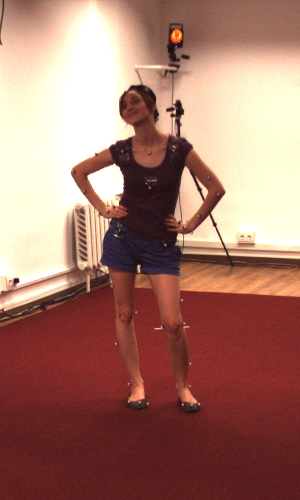
\includegraphics[width=30mm]{figures/h36_mocap.png}

    \caption{Image from Human3.6 Dataset \cite{H3.6} of subject wearing \ac
        {mocap} markers}

    \label{fig:h36_mocap}

\end{figure}

To overcome this bottleneck, \cite{unsupervisedAdversarial} proposes
unsupervised training of a generative adversarial network by projecting the
predicted 3D pose back to 2D and minimizing its distance with the input 2D
pose. And further training a discriminator to distinguish the real 2D pose
from the projected poses. Thus removing the need for any explicit 3D
annotations besides 2D poses that are either manually labeled or obtained
using 2D \ac{hpe} models. RepNet \cite{repnet} trains an adversarial
network without 2D-3D correspondences in a weakly supervised manner.
Moreover, it also does not require camera parameters to project the 3D pose
but learns to predict them. Thus enabling better generalization to more
diverse data with unknown cameras and poses.

To test the maximum capability of Pose Lifting networks, \cite{amazon1}
proposes a combination of unsupervised and adversarial learning that mainly
leverages the property of \textit{plane-invariance}. It is the property
that 2D projections of a 3D pose from different camera viewpoints, when
lifted should produce identical and the original 3D pose. In this method,
the predicted 3D pose is rotated in random angles and is reprojected to 2D
in a different \ac{pov}. A discriminator is then used to evaluate if this
new 2D pose is in the possible pose distribution which is learned from 2D
pose datasets alone. These steps are redone in reverse order to obtain the
original 2D input. This cycle provides three intermediate representations
of the single 2D input that the models learn from. Additionally, this
approach exploits the temporal consistency in the datasets as well as
integrates a domain adaptation network to learn from different datasets and
distributions to achieve comparable results to that of the methods that
require more supervision.

\subsection{Multimodal Representation Learning}

\label{section:multimodal_representation_learning}

Another interesting approach is training \ac{vae}s using multiple
modalities like images, poses, depth maps \cite{CrossingNets, crossmodal,
    MMVAE,HandDisentangled}. \ac{mvae}s learn representation from different
modalities in the same latent space. True multimodal learning needs to
fulfill 4 criteria as follows: i) \textit{Latent Factorization} - Implicit
factorization of latent space into private, shared subspaces based on
modality as illustrated in the figure[\ref{fig:criteria}]. ii) \textit
{Coherent Joint Generation} - Coherence in generations of different
modalities from the same latent value with respect to the shared aspects of
the latent. iii) \textit{Coherent Cross Generation} - Generation of one
modality conditioned on data from different modality while preserving the
similarity between them. iv) \textit{Synergy} Enhancement in generation
quality of one modality as a result of learning representations of
different modalities.

\begin{figure}[!h]

    \centering

    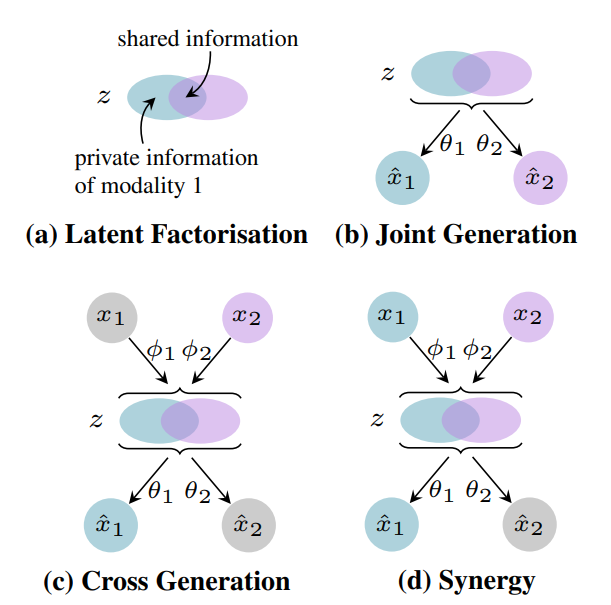
\includegraphics[scale=0.4]{figures/criteria.png}

    \caption{Criteria for Multimodal Generation \cite{MMVAE}}

    \label{fig:criteria}

\end{figure}

\ac{mmvae} proposed by \cite{MMVAE} fulfills all 4 of the above-mentioned
criteria learning representations of image and text data, while other
approaches focus on leveraging specific advantages of multimodal learning.
Consider the cross-modal learning for 3D Hand Pose Estimation proposed by
\cite{crossmodal}. It involves training an encoder-decoder pair to learn
image representation, and another such pair to learn 3D hand pose
representations in the same latent space. This training procedure focuses
on cross-generation and synergy. That is, using the shared latent space of
the image and pose representations, the \ac{rgb} image encoder combined
with the pose decoder can generate 3D poses and vice versa while preserving
the commonality between the conditioned and the generated data. With this
approach, it is possible to train a \ac{vae} for 3D \ac{hpe} from \ac{rgb}
images without explicit intermediate stages like the earlier mentioned
cascading approaches. Making it more efficient and fast for both training
and inference without compromising the modularity offered by cascading
approaches.

%TODO add exemplar methods

\section{Related Work - A closer look}
\label{section:Related Work}

In this section, works that are directly related to the thesis are discussed in more detail. Some are the best examples of their kind and have already been discussed thoroughly. The basic idea of the thesis is to learn 3D \ac{hpe} just from 2D pose data without using 3D ground truth in any shape or form. Thus developing a method that can exploit the huge amounts of 2D pose data that can be generated using state of the art 2D pose networks on diverse images from the real world. The following approaches uses weakly supervised or unsupervised approaches to accomplish the same. These serve as the inspiration for many of the choices taken in this thesis and also help understand the possibilities of reducing the need for explicit 3D supervision.

% FIXME better cite instead of just using numbers
To the best of knowledge acquired during the period of the thesis, \cite{can3dpose, amazon1, unsupervisedAdversarial, c3dpo} are the main approaches that do not use 3D supervision in any way. While \cite{repnet, weaklymultiple} are among the main appraoches the use 3D supervision to train the discriminator alone. The approaches that are not mentioned are either the approaches the above mentioned are built up or have been missed during the literature study.

\cite{unsupervisedAdversarial, can3dpose, amazon1} can be viewed as a series of approaches that are built on one another in the same order. They take 2D poses as the input and learn to predict the depth offset for each joint to reconstruct 3D. Out of the three Ching et al. \cite{amazon1}, using the plane invariance, geometric self-supervision and adversarial learning as discussed in \ref{sec:Research area introduction}, achieves the \ac{sota} results compared to fully supervised methods and also present ways to use domain adaptation network, temporal consistancy to further integrate more datasets and improve the performance. Thus directly address the hudles of scaling the 3D \ac{hpe} network to the real world. However, they also ackwoldge the fact that most of the prediction made by \ac{sota} 2D \ac{hpe} model on real world images had missing joints. Since the proposed approaches only predict the depth of every joint, the error from the 2D input pose is directly propogated to the 3D prediction. More importantly, it is not possible to use most of the data that is generated from 2D pose models. Hence it is very crutial to handle the problem of \textit{\textbf{missing joints}} to truly unlock the potential of unsupervised learning. 

Wandt et al. \cite{repnet} also discused in \ref{sec:Research area introduction} proposes an architecture that learns to predict the whole 3D pose, while also learning the camera parameters that are used to project the predict 3D to 2D. The idea behind the camera network is to learn the view angle given pose to generalize to unknown cameras. The pose network learns to converge the predcited 2D reprojections, while using a \ac{gan} trained on \textit{\textbf{3D ground truth labels}} to supervise the predicted 3D pose. Though there is no direct error propogation from 2D input to 3D, it is important to note the problem of missing joints is not yet addressed. 

However, there another fundemental problem still persists. As mentioned in \ref{sec:background}, 2D-to-3D pose lifting is an ill-posed-inversed problem due to \textit{\textbf{depth ambiguity}} as there are multiple plausible 3D poses that gives the same 2D projection. Addressing this problem, Chen Li et al. \cite{multiplehypo} proposes a varaitional inference model inspired by the architecuture of Wandt et al. \cite{repnet} that takes 2D pose along with a \textit{latent code} to produce 3D pose. The predicted 3D pose varies according to the latent code while maintaining the same 2D reprojection. This varaitional inference of 3D pose addresses both the problems of depth ambiguity and missing joints. 

The above approach has been further improved by Chen Li et al. in \cite{weaklymultiple} to leverage adversarial training using \ac{gan} trained using 3D ground truth. Though there is no direct supervision on 3D pose, 3D data is still required to train this network. It is important to note that in the case where large amount of 3D ground truth poses are available, they can be easily exploited to generate 2D poses of large volume and it is not practical to get 3D poses in the wild to scale the models. In this thesis we try to address all the forementioned problems.

\chapter{Data}
\label{chap:data}
% \thispagestyle{fancy}
This chapter discusses the datasets used in the thesis, as well as the processing steps to make the data more learnable. The main dataset used in the thesis is \textit{Human3.6M}: Large Scale Datasets and Predictive Methods for 3D Human Sensing in Natural Environments \cite{H3.6}. Most of the related works benchmark their methods on Human3.6M and it also is freely accessible to academics on request. For further evaluation of model performance in the wild, outdoor datasets that do not have 3D ground truth such as \textit{3DPW}: 3D Poses in the Wild \cite{3dpw} would be used.

\begin{figure}[h]
    \centering
    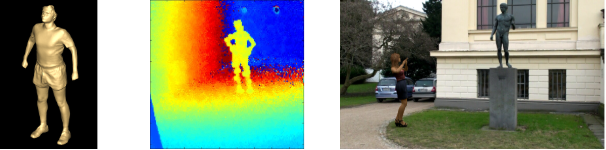
\includegraphics[width=\textwidth]{figures/h36/modlities.png}
    \caption{Full body model, depth from time of flight and mixed reality in Human3.6M dataset}
    \label{fig:h36_modality}
\end{figure}

\section{Human3.6M}
Human3.6M is a large scale indoor dataset with 3.6 million human poses collected with 4 cameras at different angles using a highly accurate maker-based \ac{MoCap} system. The dataset constitutes 15 diverse motion and actions such as eating, sitting, walking in various everyday scenarios such as, a hand in the pocket, talking over the phone, walking a dog etc. These actions are performed by 11 professional actors wearing a variety of realistic clothing. The datasets provides synchronised 2D and 3D data including full-body scans as shown in figure[\ref{fig:h36_modality}]. It also includes mixed-reality test data created using animated human models to cover huge variations of background, clothing, illumination, occlusion and camera angles. 


\section{Processing}

The methods explored by this thesis would require only images, 2D and 3D human pose from the dataset. The following are the pre-processing steps for the 2D and 3D poses.

The 3D pose in the dataset that are obtained from the marker-based \ac{MoCap} are in a global reference frame. These poses using the camera parameters, are transformed into the camera coordinate frame. For the task of predicting 3D pose from either images or 2D pose, it is unrealistic to directly estimate all the joints of the pose in a global frame. So the first step of processing would be to zero the pose w.r.t the root joint say, Pelvis. As the root is always zero, we remove it so we do not have to learn the constant joint. Removing Pelvis, 16 out of the 17 joints or keypoints remain. The 3D pose is then normalized with the mean and standard deviation of the entire training and validation poses respectively. 


\begin{figure}[h]
    \centering
    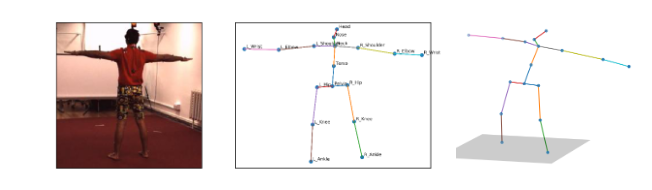
\includegraphics[width=\textwidth]{figures/h36poses.png}
    \caption{Human3.6M Pose Sample}
    \label{fig:h36_poses}
\end{figure}

The 2D pose which is obtained from the 3D pose, is also in the camera coordinate frame. The 2D pose is not zeroed as the cameras used to capture the data are not orthogonal but are perspective cameras. Zeroing the root of the 2D would eliminate the perspective information that could be important to estimate the 3D pose. The experiments to test the importance of that information is yet to be done. The root of the 2D pose is however removed to remain consistent with the 3D pose. Similar to the 3D, the 2D pose is also normalized. An image sample from the dataset with its corresponding 2D and 3D pose before normalization are illustrated in the figure[\ref{fig:h36_poses}].
% TODO update - experiments are yet to be done
% TODO link MPJPE to its explanation in other chapter or sections


The estimated poses from the networks that are trained on normalized poses are denormalized to the original scale using the same mean and standard deviation. This postprocessing step is required for getting the distance between prediction and ground truth keypoints in understandable units like millimeters. It is also necessary to denormalize for visualizing the poses, as poses normalized over all the keypoints appear heavily skewed and distorted. 




% \begin{figure}[h]
%     \begin{subfigure}{0.25\textwidth}
%     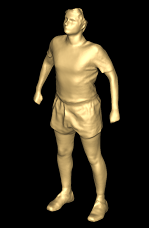
\includegraphics[height=\textwidth]{figures/h36/bodymodel.png}
%     \label{fig:h36fullbody}
%     \end{subfigure} \hspace{0.2\textwidth}
%     \begin{subfigure}{0.25\textwidth}
%     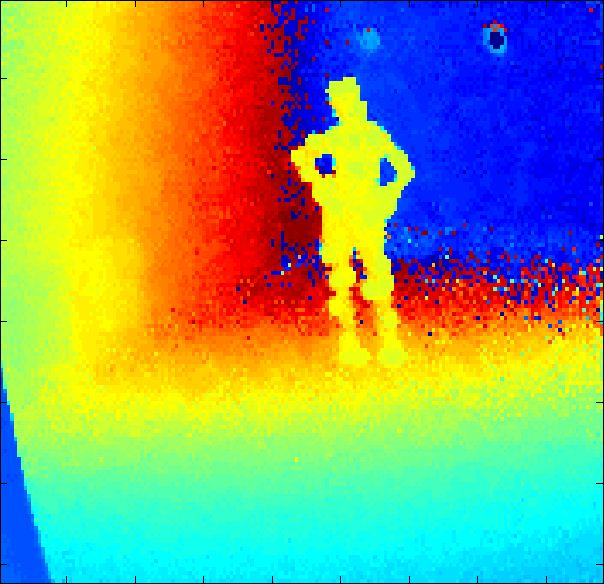
\includegraphics[height=\textwidth]{figures/h36/TOF_range.jpg}
%     \label{fig:h36tof}
%     \end{subfigure} \hspace{0.2\textwidth}
%     \begin{subfigure}{0.25\textwidth}
%     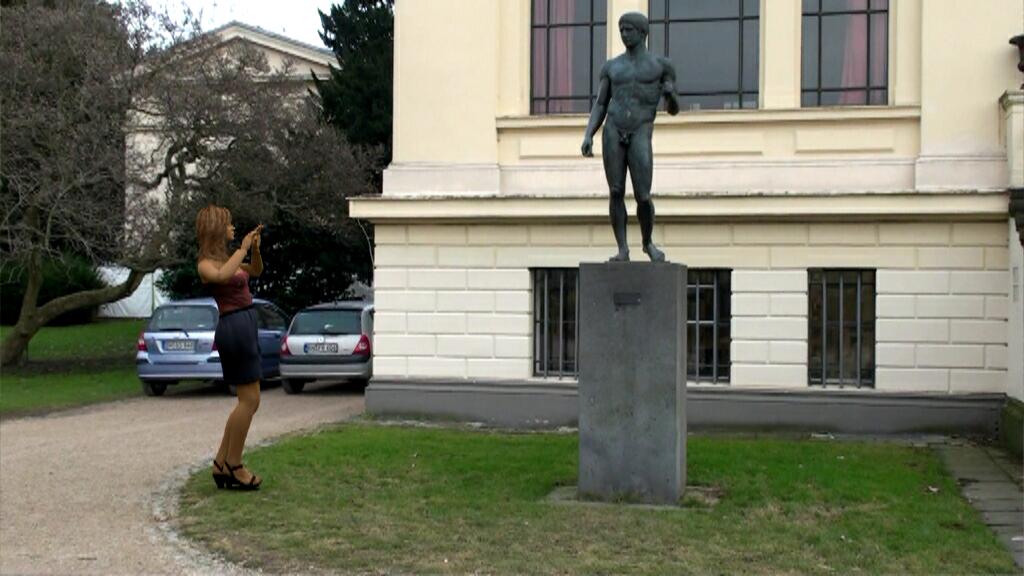
\includegraphics[height=\textwidth]{figures/h36/mixed_reality.png}
%     \label{fig:h36mixed}
%     \end{subfigure} \hspace{0.2\textwidth}
% \caption{Different modalities from Human3.6M}
% \label{fig:h36_modality}
% \end{figure}


% \begin{figure}[h]
%     \begin{subfigure}{0.25\textwidth}
%     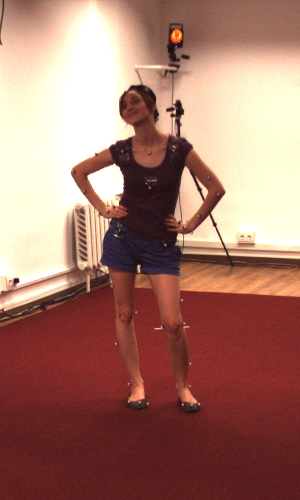
\includegraphics[height=\textwidth]{figures/h36image.png}
%     \label{fig:h36image}
%     \end{subfigure} \hspace{0.2\textwidth}
%     \begin{subfigure}{0.25\textwidth}
%     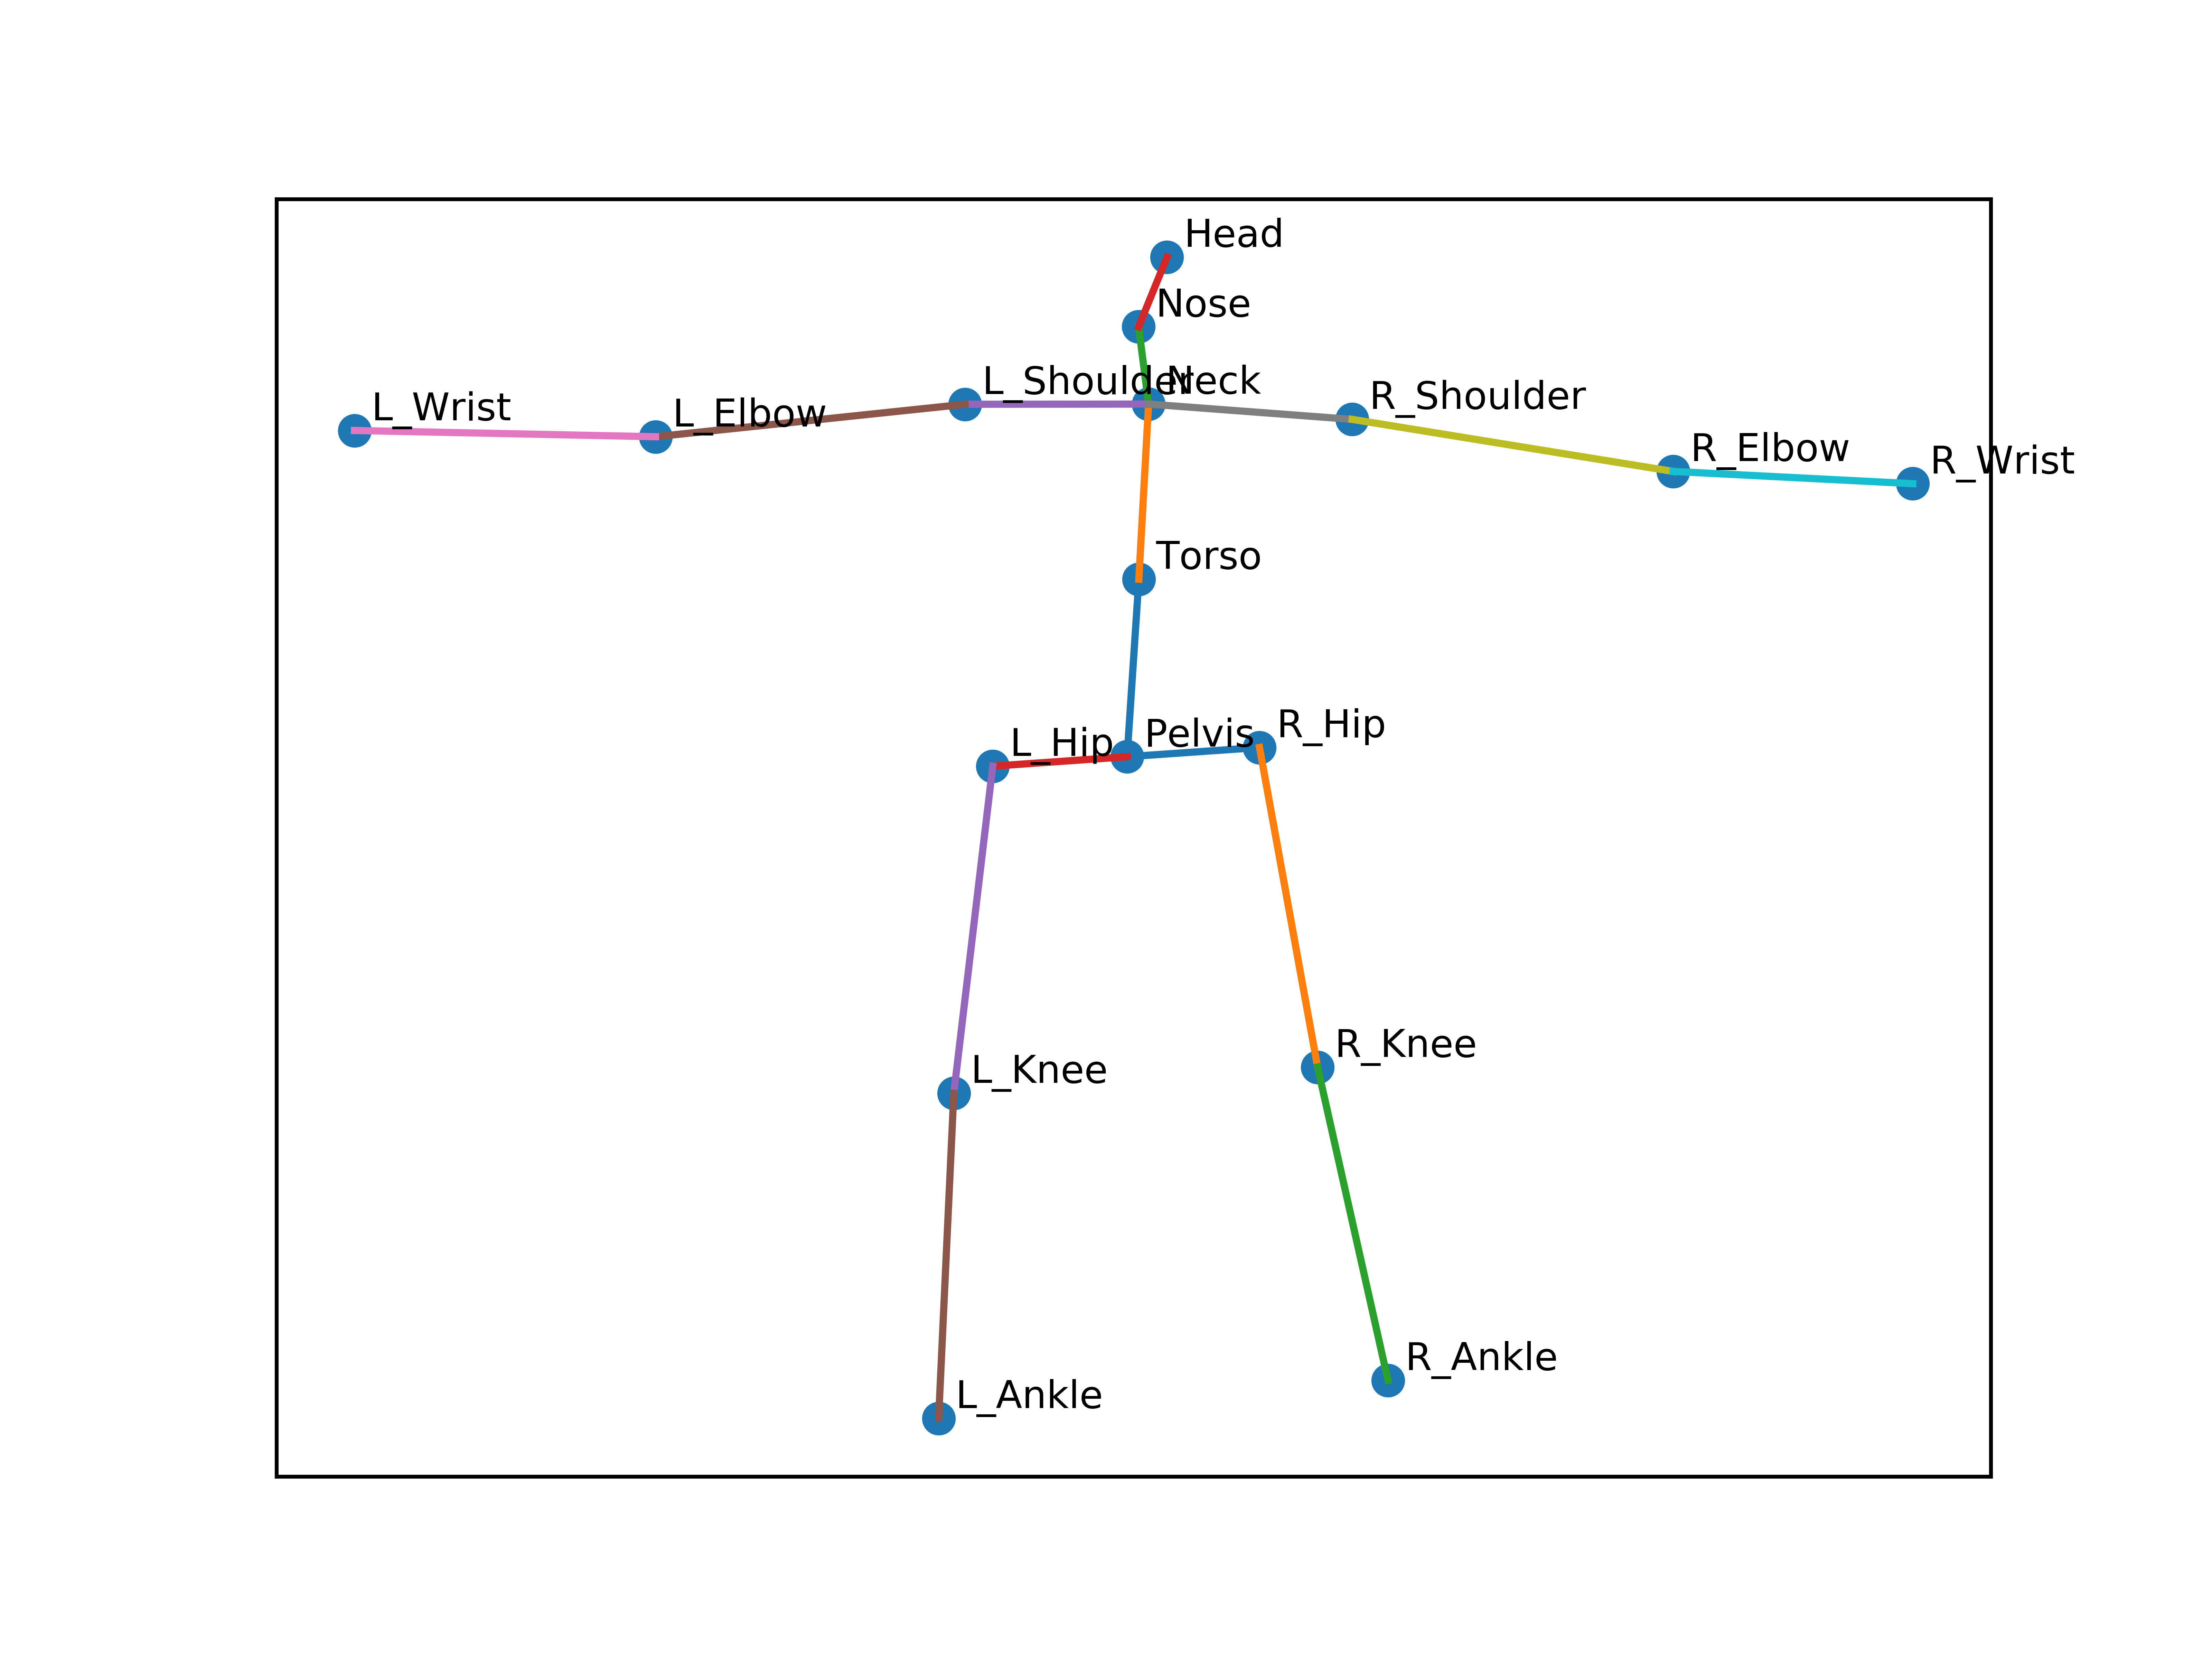
\includegraphics[height=\textwidth]{figures/h362d.png}
%     \label{fig:h362d}
%     \end{subfigure} \hspace{0.2\textwidth}
%     \begin{subfigure}{0.25\textwidth}
%     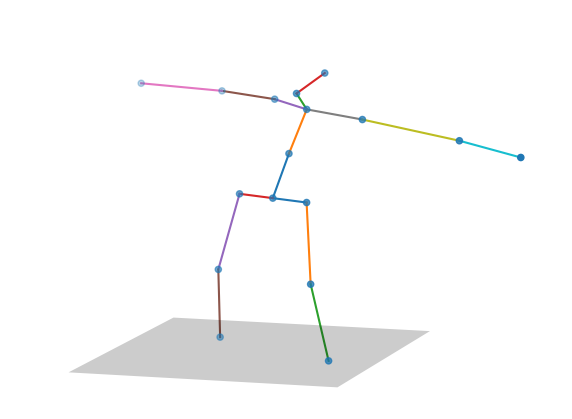
\includegraphics[height=\textwidth]{figures/h363d.png}
%     \label{fig:h363d}
%     \end{subfigure} 
% \caption{Human3.6 Pose Sample}
% \label{fig:h36_poses}
% \end{figure}
\chapter{Method}
\label{chap:method}

% \thispagestyle{fancy}
% FIXME -- change from cross model to vae-gan

This chapter presents the details and the motivation behind the design choice of the neural network such as the architecture, loss function, optimizers along with the training and evaluation procedure.

\section{Architecture}
To predict root-relative 3D pose solely using 2D poses, a hybrid network using \ac{vae} and \ac{gan} as discussed in \ref{subsec:vaeganhybrid} is employed. In contrast to the \ac{vae}-\ac{gan} hybrid introduced in \cite{autoencoding_beyond_pixels} where only the decoder acts as the generator, both the encoder and the decoder are considered as the generator in the proposed approach. In other words the encoder is also updated to maximize the probability of fooling the discriminator. The overall architecture is illustrated in the Fig \ref{fig:method_arch}. The following is the design and working of each of the components of the proposed \ac{vae}-{gan}.

\subsection{Encoder}

Adding to the explanation of \ac{vae} in \ref{subsec:vae}, the role of the encoder is to take a 2D pose as input and estimate its latent representation in the form of mean and standard deviation. The encoder consists of an upsampling layer that scales the $2 \cdot j$ dimensional input to match the number of hidden neurons of the encoding module. Where $j$ is the number of joints, here 16. The encoding module is made of $n$ residual block composed of 2 \ac{fc} layers following the related works, to allow comparison. Where $n$ is usually 1 or 2, 2 is chosen for most of the experiments. The enoding block is followed by 2 \ac{fc} layers that downsample the hidden representation to match the latent space dimension. The output of the two downsampling layers represents the mean and standard deviation of the embedding in the latent space. However in practice, the encoder is designed to predict log-variance instead of the standard deviation to have a better distribution of values and gradient. 

\subsection{Decoder}

The decoder takes the 2D pose embedding $z$ derived from the mean and log-variance predicted by the encoder and estimates the corresponding 3D pose. The reparametrization trick is used to make the process differentiable and induce variance. This is done by scaling the standard deviation obtained from the log-variance with a random sample from a unit gaussian distribution $\mathcal{N}(0,1)$. The sum of the scaled standard deviation and the mean gives the sample $z$. Similar to the encoder, the decoder consists of an upsampling layer that scales the sample $z$ of the latent space dimensions to match the number of hidden neurons in the decoding module. The decoding module is identical to the encoding module and consists of $n$ residual blocks composed of 2 \ac{fc} layers. This decoding module is followed by a \ac{fc} layer to downsample the neurons to predict 3D pose of dimension $3 \cdot j$. 

Since the 3D is projected to 2D to form the reconstruction loss, the distance between the head and the pelvis joint should approximately be of unit length as explained in \ref{processing}. To achieve this, a Tanh activation function is used to obtain the predicted 3D pose (all joints) in the range [-1, 1]. However, the length of the lower half of the pose can be longer that the upper half and usually is the case. Hence the predicted 3D pose is scaled by a factor of 1.3, the ratio of the mean length of the upper and lower halves, to enforce the length of the upper half to ~1 unit and get the best 2D re-projection.




Following the best practices from \cite{soumith2017wasserstein}, the decoder (and the encoder) which acts as the generator for the \ac{gan} is made to output 3D poses with values from [-1,1]. 
%FIXME blunder in the implementation?
All the layers use \ac{relu} activation unless specified otherwise. The decoder mimics the encoder with an upsampling layer, a decoding module, and a downsampling layer to output 3D pose of dimension .

% -1 to 1 ...scale to meet the head as 1. 
% initalization activation optimier
% at activation mention that the scaling of -1


\begin{figure}[h]
    \centering
    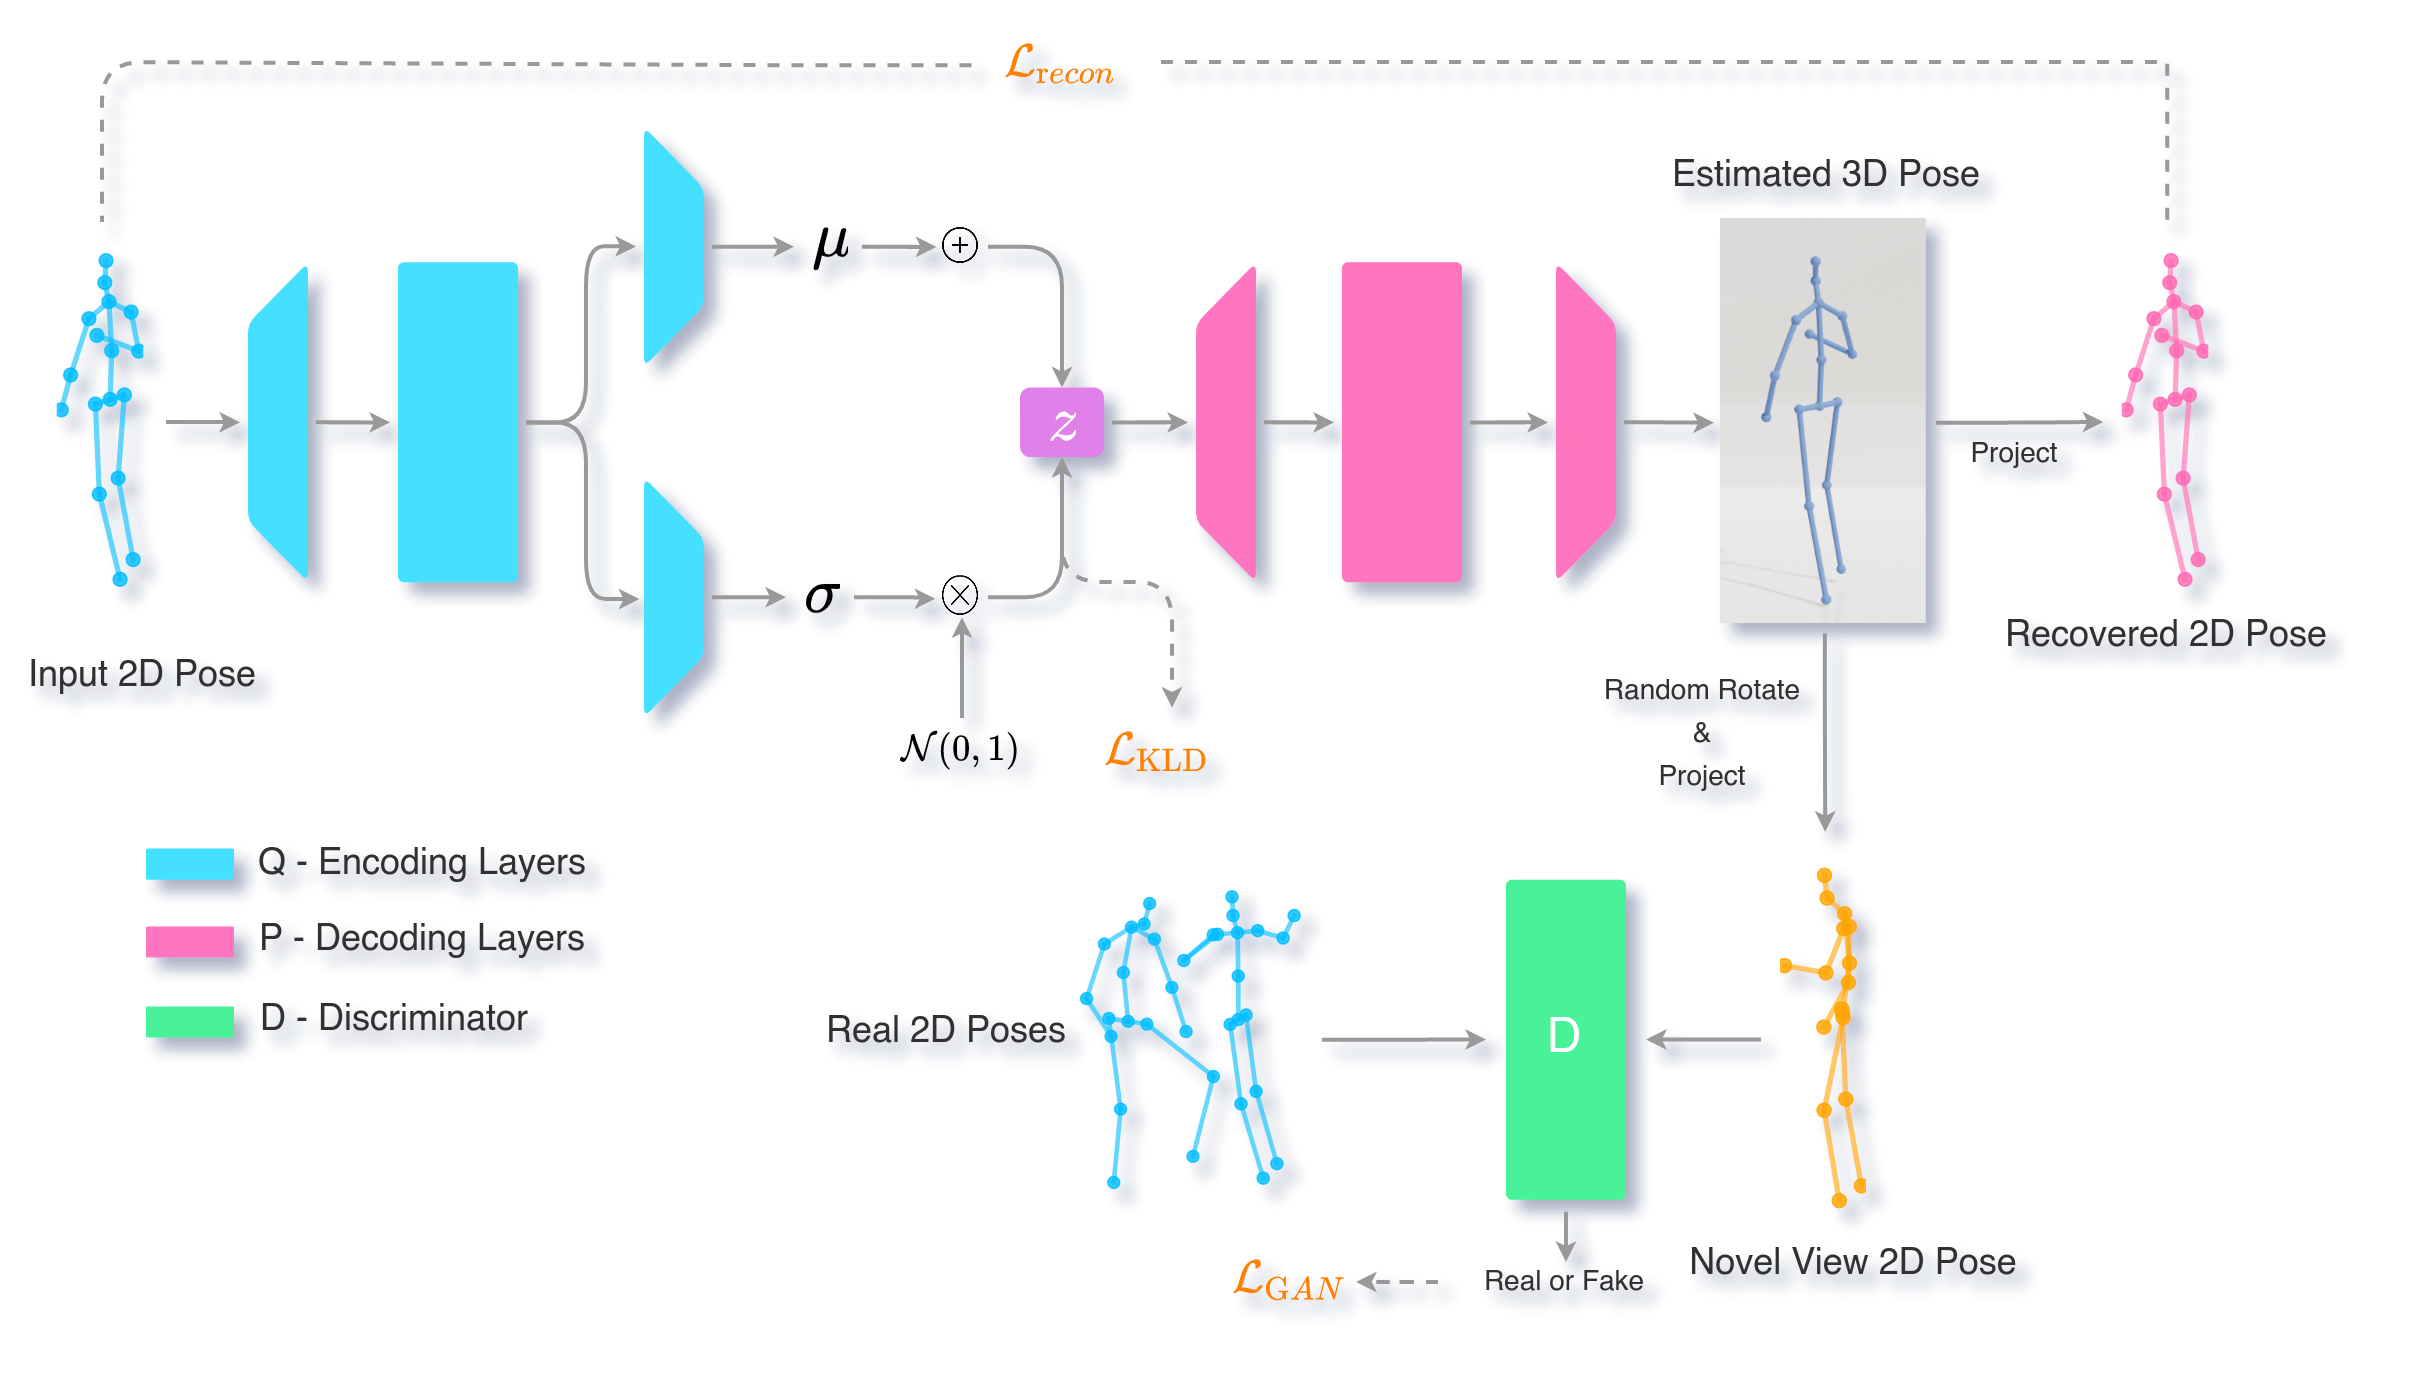
\includegraphics[width=\textwidth]{figures/arch/method_arch.png}
    \caption{Illustration of the neural architecture of the proposed method. The network components in blue, encode the 2D pose to a latent representation in terms of mean $\mu$ and standard deviation $\sigma$ of the distribution. While the components in pink, sample $z$ from this latent space and decode the corresponding 3D pose. The 3D pose is projected directly to 2D space for a contrained optimization using input 2D pose in the camera view and randomly rotated and projected for unconstrained optimization using the discriminator $D$ in a novel angle. The data that contributes to the loss function in orange, are mapped with a dotted line.  
    }
    \label{fig:method_arch}
\end{figure}


\subsection{Discriminator}%FIXME -- \subsection{Image \ac{vae}}
The discriminator following the related works also mimics the generator and takes 2D poses as input and predicts binary labels of real or false. The sigmoid activation function is used at the output layer of the discriminator.

\subsection{More on Activation functions}
beta scheduling cycling and o to 1 annealing, weighting the loss components

%FIXME
\subsection{Loss Functions}
beta scheduling cycling and o to 1 annealing, weighting the loss components

\subsection{Optimizers Functions}
beta scheduling cycling and o to 1 annealing, weighting the loss components


\section{Training Scheme}
The training scheme is similar to the standard \ac{vae} and \ac{vae}-\ac{gan} introduced in \ref{sec:Preliminary}. The discriminator is trained first for a few steps before training the \ac{vae}. First, the \ac{vae} takes the 2D pose as input and predicts the 3D pose. This predicted 3D pose is first reprojected to 2D to train the \ac{vae} and then randomly rotated and reprojected to a novel 2D view. This novel 2D is used as fake samples to train the discriminator. As \ac{vae} learns to improve the reprojected 2D pose, it will eventually be very close to the real samples. Using these as the fake examples will not be very useful as the decoder does the same job. Training the discriminator on a randomly rotated and reprojected 2D novel view would encourage the decoder to generate a pose that not only agrees with the input 2D pose but ensures that the other view of the 3D is also indistinguishable from the variations found in the data by fooling the discriminator. This two-view supervision leads to better 3D pose generations.

% \section{Bag of tricks} % TODO -- add tricks to make it work here or at work? -- it should be here
% \lipsum[1-10] %FIXME

\section{Evaluation Metrics} % FIXME
3D \ac{hpe} and Human3.6M in particular is mainly evaluated by \ac{mpjpe} metric. MPJPE as it abbreviates is the mean of the position estimate for all the joints of a pose. Where per-joint position estimate is nothing but the euclidian distance (usually measured in mm) between the predicted joint to its ground truth.


\begin{figure}[h]
    \centering
    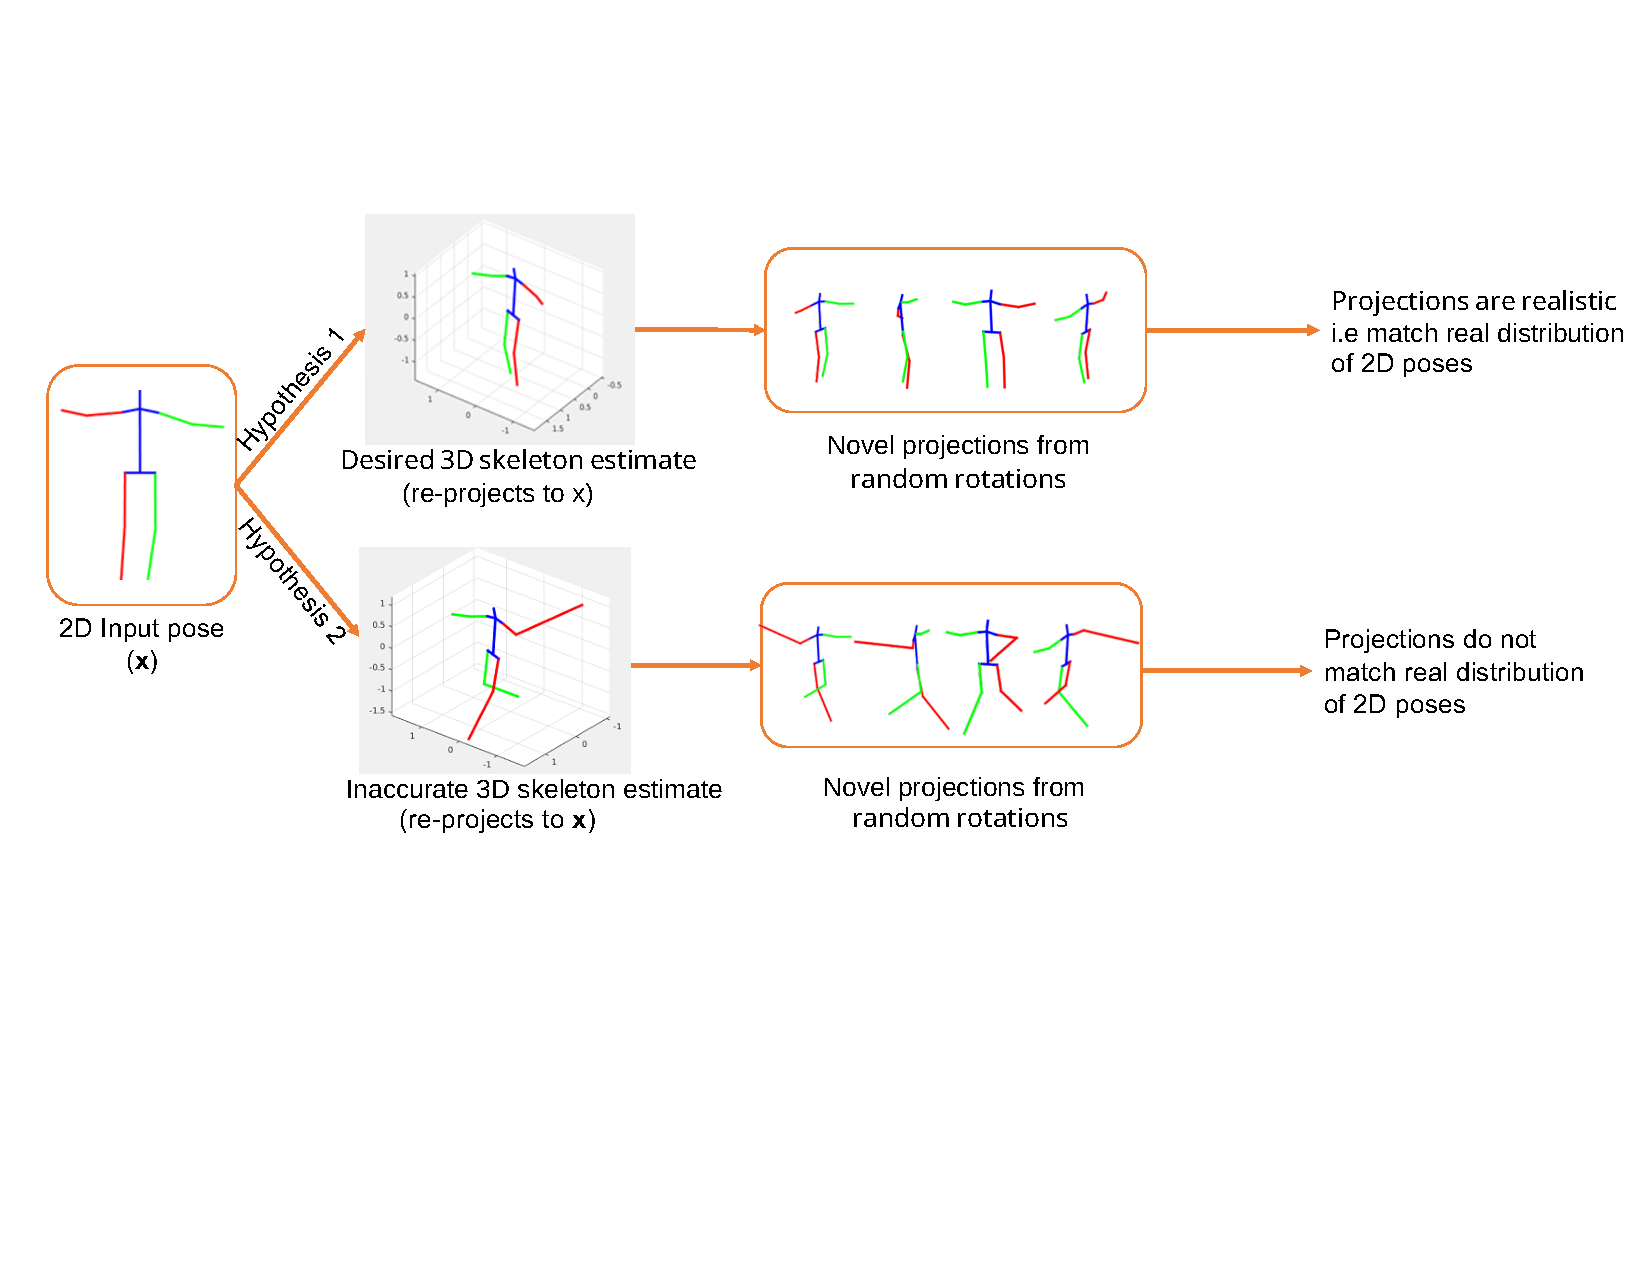
\includegraphics[width=\textwidth]{figures/h36_viz/novel_view_contraint.pdf}
    \caption{Illustration of the architecutre and loss flow in the proposed approach.}
    \label{fig:novel_view_constraint}
\end{figure}

% \section{more details the model prints?} % FIXME

\chapter{Experiments}
\label{chap:experiments}
This chapter includes the various techniques and hacks explored to enhance the \ac{gan} training and reasoning behind the choices that are crucial for the functioning of the method.% FIXME development details?

%TODO add wgan experiments
\section{Supervised Baseline}
To the best of the author's knowledge, the closest work using a \ac{vae} is a cross-modal training approach in 3D hand pose estimation \cite{crossmodal}. As there is no similar approach in \ac{hpe} using a \ac{vae}, a supervised model using just a \ac{vae} and 3D ground truth pose data is implemented. This is to verify the feasibility of a \ac{vae} and find a set of hyperparameters that worked well for the H3.6M dataset under the supervised setting. This served as a baseline over which an unsupervised \ac{gan} was built upon. Hyperparameters such as the number of neurons in the layers, the number of residual blocks $n$, dimensions of the latent space, etc are taking as reference.

\section{Unsupervised GAN}
Building upon the supervised \ac{vae}, the proposed architecture is built. The following choice is kept standard for most of the experiments and could be used to reproduce the results. All the layers are made of 1024 neurons. The encoder and the decoder are made of 1 residual block each ($n = 1$) while the discriminator is made of 2. This is to keep the capacity of the generator and the discriminator similar. Various forms of scaling the 2D poses are experimented with to make the cycle of lifting and projection smooth. The scaling mentioned in the preprocessing section where the distance between the root joint and head worked the best. %TODO is this need? is it enough? 

\section{Bag of Tricks}
\label{sec:bag_of_tricks}
The following techniques to improve the \ac{gan} training and the reasoning behind their importance are elaborated in papers such as \cite{soumith2017wasserstein,goodfellow2014generative,openaigan2wgan,improved_gan}. The important hacks or tricks from these papers and other sources are compiled in \cite{gan_hacks} and are wildly adopted in the field. Since the majority of the work in the field is on images, some of these tricks do not help and sometimes even hurt the training. These ticks along with the pre-processing steps mentioned in \refsec{sec:processing} are critical for proper training of the network. The tricks are as follows. %TODO correct when changed to experiments
 
\paragraph{Normalizing Inputs} 
It is common practice to normalize the inputs before training a neural network. When it comes to \acp{gan}, the output of the generator is the input of the discriminator. Hence it is suggested to normalize the images between [-1,1] by using a Tanh activation function at the output layer of the generator. This is another motivation behind predicting the poses in the range [-1,1] and then scaling the make the upper half of the pose to unit length.

\paragraph{Modified Loss function}
The theory the generator component of the \ac{gan} loss \ref{eqn:gan_loss}, $log(1-D(G(z)))$ is minimized. As explained in \refsec{subsec:gan}, it is replaced with maximizing $log(D(G(z)))$ as the former leads to vanishing gradients early on during the training. This is referred to as the $-logD$ trick. In practice, the labels for fakes are flipped as reals while training the generator, since the goal is to make the generator's output real according to the discriminator. And as the \ac{bce} loss \ref{eqn:loss_bce} which has a negative magnitude in its formulation is used, maximization is achieved while minimizing the loss during training. Note that the generator variable $G(z)$ in our training procedure is actually $P(Q(\textbf{x}))$. 

\paragraph{Spherical Latent Space}
Sample $z$ from a spherical distribution instead of uniform distribution. Doing interpolation along the great circle \ref{fig:great_circle} rather than a straight line from sample A to sample B. This spherical linear interpolation prevents the divergence of samples from the model's prior distribution and produces output with better features.

\begin{figure}[h] 
    \centering
    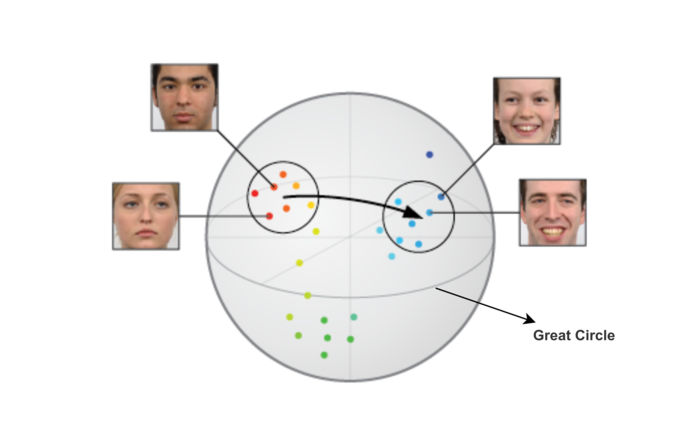
\includegraphics[width=\textwidth]{figures/background/sphericalZ.png}
    \caption{Illustration of the sampling from the great circle. Image source \cite{spherical_sampling}}
    \label{fig:great_circle}
\end{figure}

\paragraph{BatchNorm}
Training the \ac{gan} using separate batches of real and fake data without mixing them. And perform instance normalization when batch normalization is not possible.

\paragraph{Avoid Sparse Gradients}
Sparse gradients affect the training stability of the \ac{gan}. Hard functions like hard- \ac{relu}, Max Pooling that have sparse gradients should be avoided. Instead, Leaky-\ac{relu} work well for both the generator and the discriminator. And average pooling or convolution layers with stride are better for downsampling or upsampling.

As mentioned previously Tanh and Sigmoid activations are used for the output layers of the generator and the discriminator respectively. For all the remaining layers Leaky-\ac{relu} was tried and good results were observed. Experimenting with other combinations of activation functions, using Mish activation function \cite{mish} for the \ac{vae} and Leaky-\ac{relu} for the discriminator is found to give small but noticeable improvement to the performance.

Based on the choice of activation, Kaiming He initialization with Leaky-\ac{relu} non-linearity is used for all the layers.

\paragraph{Label Smooting}
The label smoothing technique mentioned in \cite{gan_hacks} is by replacing the binary labels for real and fake i.e 1, 0 with random numbers, between 0.7 and 1.2 and 0.0 to 0.3 respectively. However, there are different ways of doing smoothing. These include random/non-random, one-sided/two-sided, only for discriminator/both networks. Only the real labels are smoothed for both the discriminator and the generator in the experiments. 
% FIXME REDO mistake in implementation label smoothing only for D, not for G

\paragraph{Label Flipping}
The other way of making the labels noisy for the discriminator to prevent it from being too strong is by flipping labels during the discriminator training. Real labels are changed to fake and vice-versa occasionally to confuse the discriminator. 

This had some effect during the initial phase of the training but is not observed to directly affect the quantitative results and hence and kept inactive for simplicity.
% FIXME REDO experiment

\paragraph{GAN Model Choice} 
As training \acp{gan} is notoriously difficult, the most explored and studied variant DCGAN (Deep Convolutional \ac{gan}) is suggested to be used. The next best approach is to use hybrid models that use \ac{kld} or a combination of \ac{vae} and \ac{gan}. Since it is not desired to use convolutional layers in lifting networks, the proposed method is already following the best alternative.


\paragraph{Optimizer choice}
The best configuration of optimizers is Adam for the generator and SGD for the discriminator. However, this combination made the models diverge and has severely affected the training of the proposed method. Hence Adam is chosen for both the networks.

\paragraph{Noisy Inputs}
Adding noise to inputs and decaying over time helps the training. The 2D poses were added random noise in different scales but improvements were not noticeable in the basic experiments. 

\paragraph{Training Discriminator More}
To consistently get good feedback from the discriminator, it is ideal to keep always keep the discriminator at good performance. To achieve this, the discriminator is iterated $n$ times before every iteration of the \ac{vae}. However, $n$ is set to 1 as the benefit could not be seen in the initial observations.

\paragraph{Dropout}
Adding additional noise to the generator using dropout with $p=0.5$ during training and test time \cite{gan_dropout}. The discriminator uses dropout with $p=0.5$. But it is observed that adding dropout layers hurt \acp{vae} and $p=0.2$ was found to have a good trade-off. 

% \subsection{Model Summary}
% TODO wgan experiments 
% \section{Implementation}

% \lipsum[1] % FIXME
% \subsection{Monitoring}
% \lipsum[1] % FIXME

% \paragraph{use RL stability tricks} Not explored in this thesis. % TODO move to future

%TODO include flipping

\chapter{Experiments}
\label{chap:experiments}

%TODO add wgan experiments
\section{Supervised Baseline}
To the best of the author's knowledge, the closest work using a \ac{vae} is a cross-modal training approach in 3D hand pose estimation \cite{crossmodal}. As there is no similar approach in \ac{hpe} using a \ac{vae}, a supervised model using just a \ac{vae} and 3D ground truth pose data is implemented. This is to verify the feasibility of a \ac{vae} and find a set of hyperparameters that worked well for the H3.6M dataset under the supervised setting. This served as a baseline over which an unsupervised \ac{gan} was built upon. Hyperparameters such as the number of neurons in the layers, the number of residual blocks $n$, dimensions of the latent space, etc are taking as reference.

\section{Unsupervised GAN}
Building upon the supervised \ac{vae}, the proposed architecture is built. The following choice is kept standard for most of the experiments and could be used to reproduce the results. All the layers are made of 1024 neurons. The encoder and the decoder are made of 1 residual block each ($n = 1$) while the discriminator is made of 2. This is to keep the capacity of the generator and the discriminator similar. Various forms of scaling the 2D poses are experimented with to make the cycle of lifting and projection smooth. The scaling mentioned in the preprocessing section where the distance between the root joint and head worked the best. %TODO is this need? is it enough? 

The results presented in the following sections are after training the networks for $\sim$400 epochs (~5.5 hours) on approximately 300,000 2D poses with a batch size of 2560 on an Nvidia Titan X. The input poses are flipped with a probability of 0.5. The model takes 16 joints as the output where the root is added at the origin for validation. The proposed architecture consists of 1024 hidden units per linear layer and 51 latent dimensions. Both the \ac{vae} and the discriminator are trained using Adam optimizer with default hyperparameters and with a learning rate of 2e-4. The gradient norms of the discriminator are clipped to 1 when training the discriminator. While training the generator the gradient norms are clipped to 2 for all the models while the gradient values are clipped to 1000.

One of the challenging parts is finding the optimal weights for each of the terms in the triplet loss. The loss coefficients $\lambda_{recon}$, $\lambda_{\acs{kld}}$, $\lambda_{disc.}$ are set to 1, 0.001, 0.001 respectively. The higher weight is motivated by 2 reasons. $\lambda_{recon}$ refers to the constrained optimization and irrespective of how realistic it is, projection loss is desired to be consistently low to get better \ac{mpjpe}. That leads to the other reason that the quantitative results are given higher importance.
%TODO add loss standardization values to kld

The values of $\lambda{\acs{kld}}$ and $\lambda{disc.}$ can be tuned according to the task at hand based on how well the poses are to be clustered or how important it is to reject poses that are not realistic. The $\beta$ value for the \ac{vae} is cycled from 0 to $\lambda_{\acs{kld}}$ every 40 epochs. While keeping it constant at $\lambda_{\acs{kld}}$ for 10 epochs with a 10 epoch warmup at the beginning of the training.

\section{Quantitative Results}

The results obtained by the networks with the above configuration in addition to the choices mentioned in \ref{chap:method} are summarized in Table \ref{table:result_zv}. The summaries of the models are provided in appendix \ref{chap:summaries} to help reproduction.

\begin{table}[htb!]
    \centering
    \begin{tabularx}{\linewidth}{XXX}%{llcc}
        \toprule
        Supervision  & Algorithm                               & Error (mm) \\
        \midrule \midrule
        Full         & Martinez \etal \cite{MartinezHRL17}     & 37.1       \\
                     & Chen \etal \cite{multiplehypo} (SH, MH) & 42.6       \\
        \midrule
        Weak         & Wandt \etal \cite{repnet}               & 38.2       \\
                     & Drover \etal \cite{can3dpose}           & 38.2       \\
                     & Chen \etal \cite{weaklymultiple} (SH)   & 48.7       \\
                     & Chen \etal \cite{weaklymultiple} (BH)   & 31.6       \\
        \midrule
        Unsupervised & Ching \etal \cite{amazon1}              & 58         \\
                     & Ching \etal \cite{amazon1} (AD) (TD)    & 51         \\
                     & \textbf{Ours}                           & 52.4       \\
                     & \textbf{Ours} (BH)                        & 50         \\
        \bottomrule
    \end{tabularx}
    \caption{}
    \label{table:result_zv}
    \vspace{-3ex}
\end{table}

\textbf{SH} refers to the results using 2D Stacked Hourglass detections as input. These detections are noisy and directly affects the predictions of the model. And \textbf{DA} refers to using Domain Adaptation network to include additional datasets and \textbf{TD} denotes the use of temporal data. It is important to note that the proposed unsupervised method and the one presented in \cite{amazon1} are the only methods that do not predict the scale of the 3D pose due to the processing technique.


\begin{table}[h]
    \centering
    \footnotesize
    % \hspace{-3mm}
    % \tabcolsep=0.1mm
    \begin{tabularx}{\textwidth}{XXXXXXXX}
        \toprule
        R\_Hip & R\_Knee & R\_Ankle    & L\_Hip   & L\_Knee  & L\_Ankle    & Torso    & Neck \\
        \hline
        58.01  & 61.42   & 81.97       & 52.45    & 60.13    & 92.82       & 44.78    & 25.43 \\
        &&&&&&&\\
        Nose   & Head    & L\_Shoulder & L\_Elbow & L\_Wrist & R\_Shoulder & R\_Elbow & R\_Wrist\\
        \hline
        33.39  & 46.29   & 30.48       & 55.72    & 80.84    & 33.53       & 59.23    & 80.05\\
        \bottomrule
    \end{tabularx}
    \caption{Average per joint position error (in mm) for each \textbf{joint} under Protocol $\#2$ using 2D ground truth.}
    \label{table:pjpe}
\end{table}

\begin{table}[h]
    \centering
    \footnotesize
    % \hspace{-3mm}
    % \tabcolsep=0.1mm
    \begin{tabularx}{\textwidth}{XXXXXXXX}
        \toprule
        Directions & Discussion& Eating& Greeting& Phoning& Photo& Posing& Purchases \\
        \hline
        44.37  & 45.14   & 56.64       & 48.15    & 56.47    & 45.06       & 47.33    & 71.30  \\
        &&&&&&&\\
        Sitting& SittingDown& Smoking& Waiting& WalkDog& Walking& WalkTogether& \\
        \hline
        72.08  & 55.01   & 52.47       & 47.37    & 47.51    & 49.53       & 44.61    &  \\
        \bottomrule
    \end{tabularx}
    \caption{Average MPJPE (in mm) for each \textbf{action} under Protocol $\#2$ using 2D ground truth.}
    \label{table:pjpe_a}
\end{table}

The best hypothesis, \textbf{BH} has improved the results by ~2.7 mm which is considerable in comparison to the equivalent gain in \cite{amazon1} using domain adaptation network with more data and temporal information. Since there is no technique to pick the best hypothesis without having access to the ground truth, the results referred to, are the ones obtained using \textbf{ZV} unless specified otherwise. 

\begin{figure}[h]
    \centering
    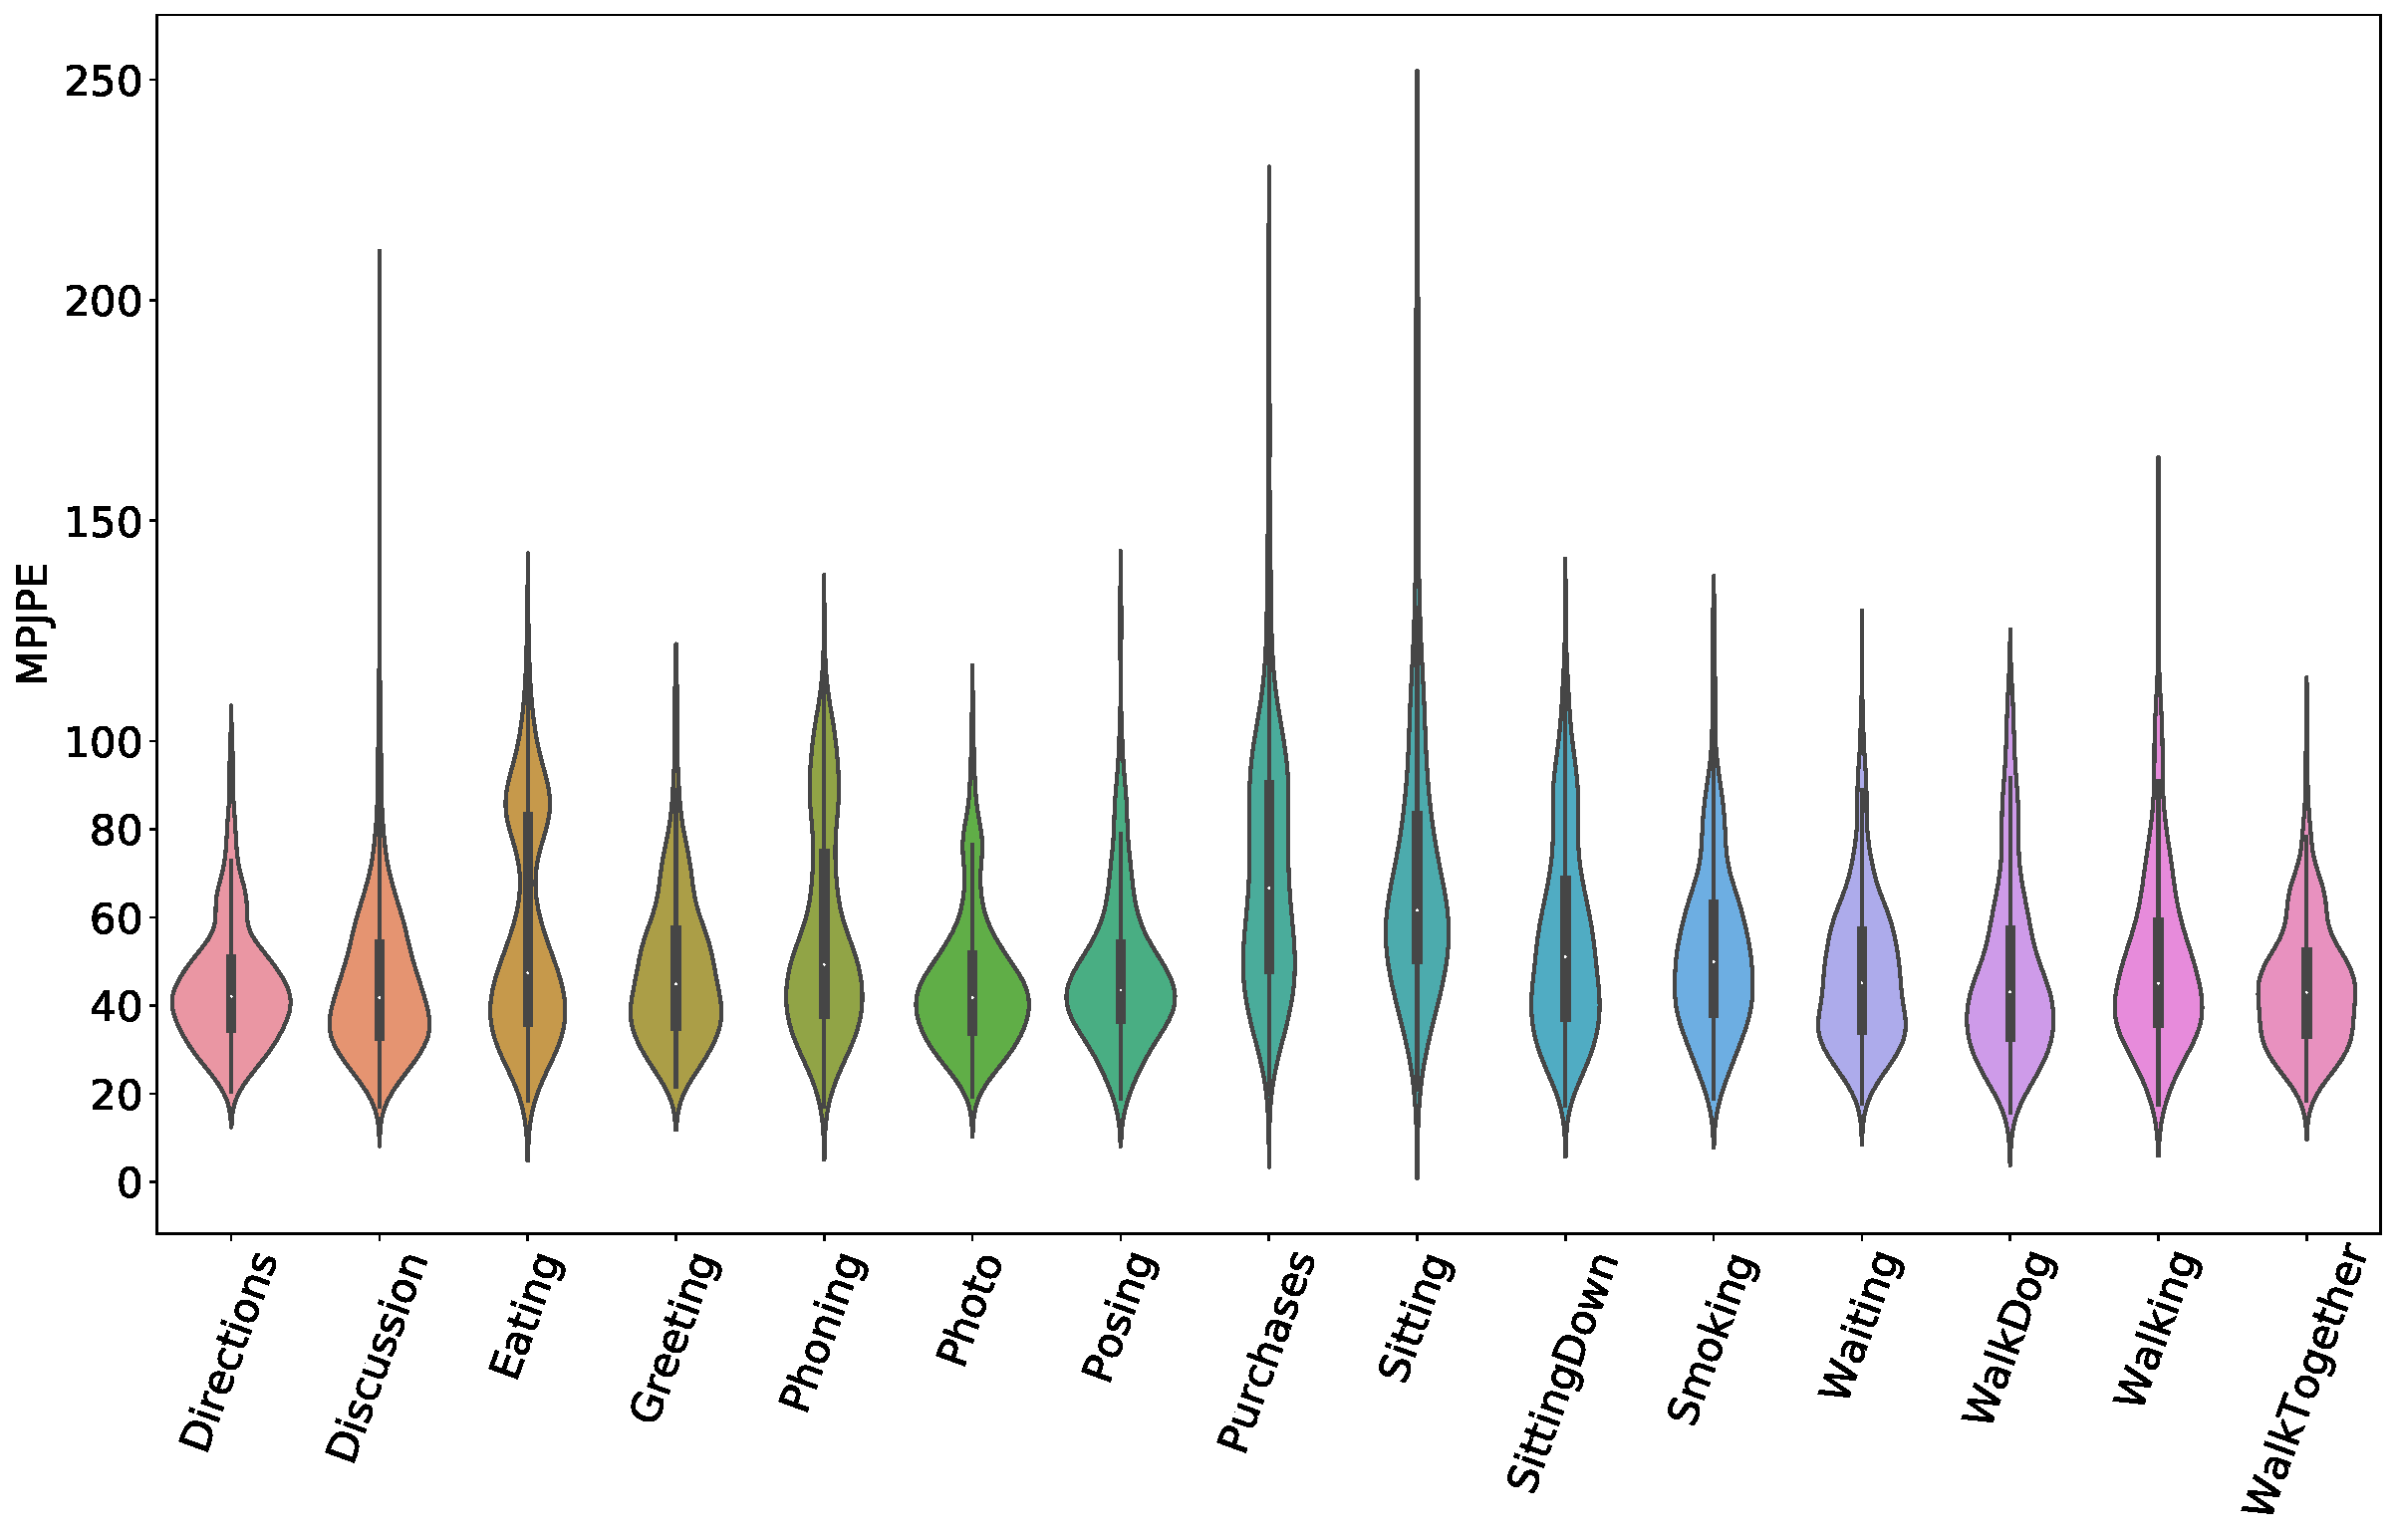
\includegraphics[width=\textwidth]{figures/results/violin_pjpe.pdf}
    \caption{Visualization of the MPJPE error distribution under Protocol $\#2$ for each action.}
    \label{fig:mpjpe_trends}
\end{figure}

The average \ac{mpjpe} errors for each action is presented in Table \ref{table:pjpe_a}, and Fig \ref{fig:mpjpe_trends} illustrates the distribution of these errors. The \ac{mpjpe} error per joint increases as we move from inner to outer joints. This can be observed in Table \ref{table:pjpe} which shows the average per joint position error. The error for the Pelvis joint is not mentioned as it is assumed to be at the origin and is always zero. The larger errors in the limb joints are due to the higher variation in their location throughout the data compared to joints like the neck or the nose. Moreover, these joints are often occluded by the person's body especially when doing actions such as sitting. The 2D projections of a pose from sitting posture is clustered to a smaller region from certain \acp{pov}. This makes it challenging to estimate the scale and depth of each joint and leads to outliers as visualized in the violin plots.

Since the data consists of an equal mix of data from different \acp{pov}, the predictions from the \ac{pov}, where the limbs are in the \ac{fov} are more informative than the other \acp{pov}. When the limbs are not in the \ac{fov}, the model learns to guess their location based on other features such as articulation or posture of the body. The effect of \ac{pov} is the possible cause of the bimodal error distribution in actions such as purchases, eating, phoning. Since the actions are hands specific, they are restricted to a particular region making the pose more predictable from one \ac{pov} and less from another. These challenges are inherent to the task of pose lifting and in many cases are challenging even for a human eye.


\section{Qualitative Results}
\subsection{Average Cases}
Since pose lifting is a tough task for humans as well, the errors around and below 50mm are usually not identifiable without 3D ground truth reference. To give a better perspective and sense of depth, 3D models are used to visualize the model predictions. Instead of handpicking predictions, poses that have errors closest to the mean of the respective action are selected and visualized in Fig \ref{fig:zv_mean}. The maximum mean \ac{mpjpe} per action as presented in table \ref{table:pjpe_a}, is not more than 75 mm and thus the predictions (in blue) are not very different from the ground truth pose (in pink). The limb joints especially the elbows and the wrist are occluded by the body in the majority of the visualized poses. Consider the 2D poses where the subject is seen in a side view, ignoring the RGB background it is quite ambiguous to say which limb is forward and which is back. The network has guessed the location of these joints to a good extent. The postures in the actions such as sitting down, sitting on a chair, etc have been predicted well.

\newcommand{\inp}[1]{figures/zv_mean/#1_inp.png}
\newcommand{\pred}[1]{figures/zv_mean/#1_pred.png}
\newcommand{\gt}[1]{figures/zv_mean/#1_gt.png}

\newif\ifreal 
% \realtrue

\begin{figure}[h!]
    \centering
    \ifreal
    \begin{subfigure}[b]{0.45\textwidth}
        \includegraphics[width=0.3\textwidth]{\inp{3493}}
        \includegraphics[width=0.3\textwidth]{\pred{3493}}
        \includegraphics[width=0.3\textwidth]{\gt{3493}}
        % \caption*{Directions - 44.44mm}
    \end{subfigure}
    \begin{subfigure}[b]{0.45\textwidth}
        \includegraphics[width=0.3\textwidth]{\inp{6422}}
        \includegraphics[width=0.3\textwidth]{\pred{6422}}
        \includegraphics[width=0.3\textwidth]{\gt{6422}}
        % \caption*{Discussion - 44.49mm}
    \end{subfigure}
    
    
    \begin{subfigure}[b]{0.45\textwidth}
        \includegraphics[width=0.3\textwidth]{\inp{14027}}
        \includegraphics[width=0.3\textwidth]{\pred{14027}}
        \includegraphics[width=0.3\textwidth]{\gt{14027}}
        % \caption*{Eating - 56.63mm}
    \end{subfigure}
    \begin{subfigure}[b]{0.45\textwidth}
        \includegraphics[width=0.3\textwidth]{\inp{74176}}
        \includegraphics[width=0.3\textwidth]{\pred{74176}}
        \includegraphics[width=0.3\textwidth]{\gt{74176}}
        % \caption*{Greeting - 49.15mm}
    \end{subfigure}
    
    
    \begin{subfigure}[b]{0.45\textwidth}
        \includegraphics[width=0.3\textwidth]{\inp{21621}}
        \includegraphics[width=0.3\textwidth]{\pred{21621}}
        \includegraphics[width=0.3\textwidth]{\gt{21621}}
        % \caption*{Phoning - 56.59mm}
    \end{subfigure}
    \begin{subfigure}[b]{0.45\textwidth}
        \includegraphics[width=0.3\textwidth]{\inp{26692}}
        \includegraphics[width=0.3\textwidth]{\pred{26692}}
        \includegraphics[width=0.3\textwidth]{\gt{26692}}
        % \caption*{Photo - 44.22mm}
    \end{subfigure}
    
    
    \begin{subfigure}[b]{0.45\textwidth}
        \includegraphics[width=0.3\textwidth]{\inp{30089}}
        \includegraphics[width=0.3\textwidth]{\pred{30089}}
        \includegraphics[width=0.3\textwidth]{\gt{30089}}
        % \caption*{Posing - 46.50mm}
    \end{subfigure}
    \begin{subfigure}[b]{0.45\textwidth}
        \includegraphics[width=0.3\textwidth]{\inp{33987}}
        \includegraphics[width=0.3\textwidth]{\pred{33987}}
        \includegraphics[width=0.3\textwidth]{\gt{33987}}
        % \caption*{Purchases - 71.16mm}
    \end{subfigure}
    
    
    \begin{subfigure}[b]{0.45\textwidth}
        \includegraphics[width=0.3\textwidth]{\inp{39416}}
        \includegraphics[width=0.3\textwidth]{\pred{39416}}
        \includegraphics[width=0.3\textwidth]{\gt{39416}}
        % \caption*{Sitting - 72.55mm}
    \end{subfigure}
    \begin{subfigure}[b]{0.45\textwidth}
        \includegraphics[width=0.3\textwidth]{\inp{94650}}
        \includegraphics[width=0.3\textwidth]{\pred{94650}}
        \includegraphics[width=0.3\textwidth]{\gt{94650}}
        % \caption*{SittingDown - 55.01mm}
    \end{subfigure}
    
    
    \begin{subfigure}[b]{0.45\textwidth}
        \includegraphics[width=0.3\textwidth]{\inp{96348}}
        \includegraphics[width=0.3\textwidth]{\pred{96348}}
        \includegraphics[width=0.3\textwidth]{\gt{96348}}
        % \caption*{Smoking - 51.98mm}
    \end{subfigure}
    \begin{subfigure}[b]{0.45\textwidth}
        \includegraphics[width=0.3\textwidth]{\inp{54005}}
        \includegraphics[width=0.3\textwidth]{\pred{54005}}
        \includegraphics[width=0.3\textwidth]{\gt{54005}}
        % \caption*{Waiting - 47.79mm}
    \end{subfigure}
    
    
    \begin{subfigure}[b]{0.45\textwidth}
        \includegraphics[width=0.3\textwidth]{\inp{55495}}
        \includegraphics[width=0.3\textwidth]{\pred{55495}}
        \includegraphics[width=0.3\textwidth]{\gt{55495}}
        % \caption*{WalkDog - 46.86mm}
    \end{subfigure}
    \begin{subfigure}[b]{0.45\textwidth}
        \includegraphics[width=0.3\textwidth]{\inp{106863}}
        \includegraphics[width=0.3\textwidth]{\pred{106863}}
        \includegraphics[width=0.3\textwidth]{\gt{106863}}
        % \caption*{Walking - 48.73mm}
    \end{subfigure}
    
    \begin{subfigure}[b]{0.45\textwidth}
        \includegraphics[width=0.3\textwidth]{\inp{109473}}
        \includegraphics[width=0.3\textwidth]{\pred{109473}}
        \includegraphics[width=0.3\textwidth]{\gt{109473}}
        % \caption*{WalkTogether - 44.00mm}
    \end{subfigure}
    \else
        \includegraphics[width=\textwidth]{example-grid-100x100pt}
    \fi
    \caption{Visualization of (left to right) the input 2D poses with RGB background for reference, the predicted 3D pose after Procrustes alignment (in blue) and the ground truth 3D pose (in pink). The aligned predictions are the ones closest to the \textbf{mean} MPJPE error of each action.}
    \label{fig:zv_mean}
\end{figure}


















\newcommand{\inp}[1]{figures/zv_fail/fails_#1_inp.png}
\newcommand{\pred}[1]{figures/zv_fail/fails_#1_pred.png}
\newcommand{\gt}[1]{figures/zv_fail/fails_#1_gt.png}


\begin{figure}[h]
    \centering
    \begin{subfigure}[b]{0.45\textwidth}
        \includegraphics[width=0.3\textwidth]{\inp{2878}}
        \includegraphics[width=0.3\textwidth]{\pred{2878}}
        \includegraphics[width=0.3\textwidth]{\gt{2878}}
        % \caption*{Directions - 44.44mm}
    \end{subfigure}
    \begin{subfigure}[b]{0.45\textwidth}
        \includegraphics[width=0.3\textwidth]{\inp{6130}}
        \includegraphics[width=0.3\textwidth]{\pred{6130}}
        \includegraphics[width=0.3\textwidth]{\gt{6130}}
        % \caption*{Discussion - 44.49mm}
    \end{subfigure}



    \begin{subfigure}[b]{0.45\textwidth}
        \includegraphics[width=0.3\textwidth]{\inp{73047}}
        \includegraphics[width=0.3\textwidth]{\pred{73047}}
        \includegraphics[width=0.3\textwidth]{\gt{73047}}
        % \caption*{Eating - 56.63mm}
    \end{subfigure}
    \begin{subfigure}[b]{0.45\textwidth}
        \includegraphics[width=0.3\textwidth]{\inp{18120}}
        \includegraphics[width=0.3\textwidth]{\pred{18120}}
        \includegraphics[width=0.3\textwidth]{\gt{18120}}
        % \caption*{Greeting - 49.15mm}
    \end{subfigure}



    \begin{subfigure}[b]{0.45\textwidth}
        \includegraphics[width=0.3\textwidth]{\inp{24801}}
        \includegraphics[width=0.3\textwidth]{\pred{24801}}
        \includegraphics[width=0.3\textwidth]{\gt{24801}}
        % \caption*{Phoning - 56.59mm}
    \end{subfigure}
    \begin{subfigure}[b]{0.45\textwidth}
        \includegraphics[width=0.3\textwidth]{\inp{26722}}
        \includegraphics[width=0.3\textwidth]{\pred{26722}}
        \includegraphics[width=0.3\textwidth]{\gt{26722}}
        % \caption*{Photo - 44.22mm}
    \end{subfigure}



    \begin{subfigure}[b]{0.45\textwidth}
        \includegraphics[width=0.3\textwidth]{\inp{31669}}
        \includegraphics[width=0.3\textwidth]{\pred{31669}}
        \includegraphics[width=0.3\textwidth]{\gt{31669}}
        % \caption*{Posing - 46.50mm}
    \end{subfigure}
    % \begin{subfigure}[b]{0.45\textwidth}
    %     \includegraphics[width=0.3\textwidth]{\inp{34930}}
    %     \includegraphics[width=0.3\textwidth]{\pred{34930}}
    %     \includegraphics[width=0.3\textwidth]{\gt{34930}}
    % \caption*{Purchases - 71.16mm}
    % \end{subfigure}
    % \begin{subfigure}[b]{0.45\textwidth}
    %     \includegraphics[width=0.3\textwidth]{\inp{90950}}
    %     \includegraphics[width=0.3\textwidth]{\pred{90950}}
    %     \includegraphics[width=0.3\textwidth]{\gt{90950}}
    %     % \caption*{Sitting - 72.55mm}
    % \end{subfigure}
    \begin{subfigure}[b]{0.45\textwidth}
        \includegraphics[width=0.3\textwidth]{\inp{43450}}
        \includegraphics[width=0.3\textwidth]{\pred{43450}}
        \includegraphics[width=0.3\textwidth]{\gt{43450}}
        % \caption*{SittingDown - 55.01mm}
    \end{subfigure}



    \begin{subfigure}[b]{0.45\textwidth}
        \includegraphics[width=0.3\textwidth]{\inp{98756}}
        \includegraphics[width=0.3\textwidth]{\pred{98756}}
        \includegraphics[width=0.3\textwidth]{\gt{98756}}
        % \caption*{Smoking - 51.98mm}
    \end{subfigure}
    \begin{subfigure}[b]{0.45\textwidth}
        \includegraphics[width=0.3\textwidth]{\inp{101351}}
        \includegraphics[width=0.3\textwidth]{\pred{101351}}
        \includegraphics[width=0.3\textwidth]{\gt{101351}}
        % \caption*{Waiting - 47.79mm}
    \end{subfigure}



    \begin{subfigure}[b]{0.45\textwidth}
        \includegraphics[width=0.3\textwidth]{\inp{105002}}
        \includegraphics[width=0.3\textwidth]{\pred{105002}}
        \includegraphics[width=0.3\textwidth]{\gt{105002}}
        % \caption*{WalkDog - 46.86mm}
    \end{subfigure}
    \begin{subfigure}[b]{0.45\textwidth}
        \includegraphics[width=0.3\textwidth]{\inp{106047}}
        \includegraphics[width=0.3\textwidth]{\pred{106047}}
        \includegraphics[width=0.3\textwidth]{\gt{106047}}
        % \caption*{Walking - 48.73mm}
    \end{subfigure}


    \begin{subfigure}[b]{0.45\textwidth}
        \includegraphics[width=0.3\textwidth]{\inp{61221}}
        \includegraphics[width=0.3\textwidth]{\pred{61221}}
        \includegraphics[width=0.3\textwidth]{\gt{61221}}
        % \caption*{WalkTogether - 44.00mm}
    \end{subfigure}

    \caption{Left to right are the input 2D poses with RGB reference, the predicted 3D pose (in blue) and the ground truth 3D pose (in pink). The aligned predictions are the ones closest to the mean MPJPE error of every action.}
    \label{table:zv_fail}
\end{figure}



















\subsection{Failure Cases}

Similarly, the poses with the maximum errors (outliers) are taken for each action and visualized in Fig \ref{fig:zv_fail}. The main reason as mentioned earlier is the failure in estimating the depth or in predicting a good representation of the 2D pose for the decoder. One of the best examples of ambiguity can be seen in the visualizations where the 3D pose is very plausible, with very good 2D reprojection but with the subject facing the wrong direction. It can be observed from some of the visualizations in \ref{fig:zv_fail}, that the predicted joints are consistent with respect to each other but are away from the root joint. Note that the root joint is always added to the prediction at the origin. Since the rest of the pose is consistent it could be implied that the model failed to predict the depth of the joints properly. Consider the model predicts a 3D pose whose 2D projection is deviated from the input 2D. This error is magnified in 3D if the joint is farther away from the image. To overcome such errors, higher weight is given to the 2D reconstruction loss.

%FIXME add an example for all actions


\section{Latent Space}
A good representation of the 2D poses in the latent space not only helps the decoder to construct better 3D poses but also shows the models understanding of the pose in terms of the articulation/posture, and the \ac{pov}. Though the ZV model used to report these results is not tuned to have the best clustering, it still should learn an efficient representation to encode the 2D poses in the latent space. In order to evaluate the encoder capabilities, the test dataset consisting of $\approx 8000$ 2D poses are encoded to $51$-dimensional latent space. These embeddings $z$ are further reduced to two dimensions using \ac{umap} \cite{umap}. The clustering is computed using $50$ neighbors and $0.1$ units of minimum Euclidean distance and the reduced embeddings are visualized in Fig \ref{fig:latentspace}.

\begin{figure}[h]
    \centering
    \includegraphics[width=\linewidth]{figures/results/umap.pdf}
    \caption{Visualization of the 2D pose embeddings in the latent space using UMAP dimensionality reduction.}
    \label{fig:latentspace}
\end{figure}

The reduced $z$ are colored with respect to their action. This is not an ideal way to examine the clustering as there is significant overlap in the actions during their 'transition phase'. For example, as the data is collected as the subject performs that action, the subject would be 'standing' before 'sitting down'. Since it is not practical to label each frame, the action labels are used. Despite the overlap, patterns and clusters can be seen indicating a good representation capability of the encoder. To further evaluate the extent of clustering, 5 nearest latent neighbors of the embeddings of a few interesting poses are queried to verify if they represent common distribution. The corresponding 2D poses of these embeddings are visualized in Fig \ref{fig:neighbors}. Strong similarity can be observed among the nearest neighbors. Similarities include a set of joints having the same articulation, natural transition from one posture to another, or a different \ac{pov} of the similar pose. 

%reference c3dpo
\newcommand{\methtext}[1]{\centering\scriptsize\hspace{0.01cm}{\hspace{0.2cm}#1}\hspace{0.02cm}}
\newcommand{\inpC}[1]{figures/neighbours/#1_2d.png}


\newif\ifreal 
% \realtrue

\begin{figure}[h]
    \centering
    \ifreal
    \begin{tabular}{p{0.15\textwidth}p{0.85\textwidth}}
        \methtext{\textbf{\color[RGB]{66,154,201}Query Pose}} &
        \methtext{\textbf{\color[RGB]{66,154,201}Nearest Neighbours in Latent Space}} \\
    \end{tabular}
    \begin{subfigure}[b]{\textwidth}
        \fbox{\includegraphics[width=0.16\textwidth]{\inpC{7817}}}
        \includegraphics[width=0.16\textwidth]{\inpC{7742}}
        \includegraphics[width=0.16\textwidth]{\inpC{7123}}
        \includegraphics[width=0.16\textwidth]{\inpC{6102}}
        \includegraphics[width=0.16\textwidth]{\inpC{7752}}
        \includegraphics[width=0.16\textwidth]{\inpC{5484}}
    \end{subfigure}
    \begin{subfigure}[b]{\textwidth}
        \fbox{\includegraphics[width=0.16\textwidth]{\inpC{3418}}}
        \includegraphics[width=0.16\textwidth]{\inpC{2850}}
        \includegraphics[width=0.16\textwidth]{\inpC{6441}}
        \includegraphics[width=0.16\textwidth]{\inpC{3279}}
        \includegraphics[width=0.16\textwidth]{\inpC{7194}}
        \includegraphics[width=0.16\textwidth]{\inpC{7126}}
    \end{subfigure}
    \begin{subfigure}[b]{\textwidth}
        \fbox{\includegraphics[width=0.16\textwidth]{\inpC{7126}}}
        \includegraphics[width=0.16\textwidth]{\inpC{7264}}
        \includegraphics[width=0.16\textwidth]{\inpC{7254}}
        \includegraphics[width=0.16\textwidth]{\inpC{7386}}
        \includegraphics[width=0.16\textwidth]{\inpC{7237}}
        \includegraphics[width=0.16\textwidth]{\inpC{7108}}
    \end{subfigure}
    \begin{subfigure}[b]{\textwidth}
        \fbox{\includegraphics[width=0.16\textwidth]{\inpC{7043}}}
        \includegraphics[width=0.16\textwidth]{\inpC{3079}}
        \includegraphics[width=0.16\textwidth]{\inpC{2895}}
        \includegraphics[width=0.16\textwidth]{\inpC{3125}}
        \includegraphics[width=0.16\textwidth]{\inpC{2888}}
        \includegraphics[width=0.16\textwidth]{\inpC{2909}}
    \end{subfigure}
    \begin{subfigure}[b]{\textwidth}
        \fbox{\includegraphics[width=0.16\textwidth]{\inpC{791}}}
        \includegraphics[width=0.16\textwidth]{\inpC{5617}}
        \includegraphics[width=0.16\textwidth]{\inpC{6755}}
        \includegraphics[width=0.16\textwidth]{\inpC{826}}
        \includegraphics[width=0.16\textwidth]{\inpC{629}}
        \includegraphics[width=0.16\textwidth]{\inpC{8435}}
    \end{subfigure}
    \else
    \includegraphics[width=\textwidth]{example-grid-100x100pt}
    \fi
    \caption{The first pose in box is the query 2D pose and the following 5 2D poses are its nearest neighbors in the latent space.}
    \label{fig:neighbors}
\end{figure}
%TODO add a downstream task for embedding video sync multi-view


\section{Missing Joints}
The other important problem the proposed method addresses is the ability to handle missing points. The intuition is from the ability of the encoder to represent similar poses together in the latent space as seen in \ref{fig:neighbors}. A 2D pose missing a joint or two should still be able to tell about the posture and the view of the subject. The encoding of such incomplete poses should be closer to the means of similar pose distributions. Given the decoder can produce plausible 3D poses, lifting the incomplete 3D pose should be at least plausible if not similar to the ground truth 3D pose. Hence the network should be able to 'hallucinate' the missing joints. To evaluate this, the model is given incomplete 2D poses obtained by randomly zeroing 1 and 2 joints. The models are not trained explicitly on any incomplete poses in order to verify the above hypothesis. The \ac{mpjpe} using \ac{zv} and \ac{bh} are reported in table \ref{table:missing_joints}. As expected, there is a significant difference between \ac{zv} and \ac{bh} as there would be many possible locations for the missing joints among which the ground truth pose would be one.

\begin{table}[htb!]
    \centering
    \begin{tabularx}{\linewidth}{XXX}%{llcc}
        \toprule
        \# Missing Joints & Zero Variance (ZV) & Best Hypothesis (BH)\\
        \midrule \midrule
        0                 & 52.74         & 50.3            \\
        1                 & 79            & 53              \\
        2                 & 101           & 65              \\
        \bottomrule
    \end{tabularx}
    \caption{Results on Human3.6M in MPJPE (in mm) under Protocol $\#2$ using ground truth 2D pose with \textbf{missing joints} as input.}
    \label{table:missing_joints}
    \vspace{-3ex}
\end{table}
\chapter{Conclusions}
\label{chap:conclusions}

\section{Discussion}
%FIXME c3dpo is weakly supervised
%FIXME include new amazon paper somewhere
Previous unsupervised learning approaches for pose lifting such as \cite{amazon1} uses deep neural networks and geometric consistency to achieve results comparable to major weakly supervised approaches such as \cite{can3dpose}. They address critical problems such as making use of datasets from different distribution using additional domain adaptation networks and exploiting temporal information. These techniques made it possible to use large amounts of 2D data to learn 3D poses. However, as the authors acknowledge the \ac{sota} 2D pose networks often get few joints very wrong or miss them due to occlusions that are quite frequent in the real-world. Hence methods that are independent of the correctness of the input 2D are essential. \cite{c3dpo,weaklymultiple} are such weakly supervised methods that can handle missing joints while \cite{weaklymultiple} can also give multiple hypotheses for a given 2D pose. The proposed method tackles these problems with a unified approach by using \acp{vae} and \ac{gan} and is completely unsupervised.

The average \ac{mpjpe} using ZV, 52.74mm, is equivalent to the settings of \cite{amazon1} without additional data or temporal information, 58 mm. This is a significant improvement considering that the network is independent of the input and can handle errors including missing joints, can produce multiple hypotheses. While \cite{amazon1} uses a self-symmetry technique that requires propagating through the models twice per iteration and requires 2 more additional networks of complexity similar to the lifting network to slightly exceed the performance of the proposed network.

Though the proposed network address all the 3 major challenges of lifting networks, i.e 3D annotations, missing joints, and variational inference, the network only predicts a unit 3D pose. This restriction limits the usability of the 3D pose in some cases or requires additional algorithms to obtain the true scale in the real-world. For example, the scale of the 3D pose is not important if the task is to use the method as a vision-based \ac{mocap} solution for gaming where only the articulation of the pose is of interest to capture complex human motion. While tasks in the domain of self-driving cars, robot-human interaction, or AR/VR applications where the pose is used for interaction among the agents, 3D pose alone would not be sufficient.


\section{Future Work}

The source of the major drawback of not predicting to scale is in the processing technique to make the self-supervision simple. This problem could be addressed by extending the method to disentangle the root-relative pose prediction and global pose prediction similar to \cite{CameraDistanceAware}. 

\acp{vae} have more to offer than just predict 3D while handling erroneous inputs. Taking the inspiration from \cite{crossmodal}, the method can be upgraded from a lifting network to end to end network to predict 3D pose from Images just by swapping the encoder model. Techniques like Synergy and Cross-Generation from cross-modal training \cite{MMVAE} could be leveraged to train an unsupervised Image to 3D model faster and efficiently with the help of large 2D pose datasets.

In addition to this guaranteed improvised techniques such as using external datasets and temporal information to learn predicting temporally consistent 3D pose as presented in \cite{amazon1} would make the network more practical to use in the real world.

\section{Final Words}

Scaling the task of 3D Human Pose Estimation to the real-world is limited by the need for 3D data. This thesis presented an unsupervised learning method that learns to predict 3D pose without a need for 3D annotations in any shape or form. The method learns to lift 2D poses to 3D strictly using 2D pose data that are obtained from 2D pose estimation models. The thesis introduced standards \acp{vae} to the task of pose lifting for the first time. This generative model is trained using \ac{gan} and self-supervision techniques. The ability of the proposed method to handle incomplete and erroneous data without explicit training is shown. The thesis also shows the capacity of the model to learn a strong representation of the pose that could be used for other applications such as human-centric multi-view video synchronization. This thesis has considerably improved the \ac{sota} in unsupervised 3D Human Pose Estimation and lays the foundation for new ways to tackle the problem.






\include{content}

\newpage
\addcontentsline{toc}{chapter}{References}
\printbibliography

\newpage
\appendix
\newpage
\etocdepthtag.toc{mtappendix}
\etocsettagdepth{mtchapter}{none}
\etocsettagdepth{mtappendix}{subsection}
\etoctocstyle{1}{Appendix - Contents}
\tableofcontents
\newpage


\chapter{First Appendix}
This is only slightly related to the rest of the report


\chapter{Second Appendix}
this is the information


\newpage
% This is the last page of the document
\thispagestyle{empty}
\AddToShipoutPictureBG*{%]
    \AtPageLowerLeft{%
        \includegraphics[width=1.0\paperwidth]{setup/img/kth-footer.png}
    }%
}

\PlaceText{20mm}{282mm}{\color{white}\fontsize{12}{0}\sffamily www.kth.se }


\end{document}
